% !TeX spellcheck = en_GB
\documentclass[usenames,dvipsnames,aspectratio=169]{beamer}
\usetheme{Szeged}
\usecolortheme{beaver}
\usepackage{multimedia}
\usepackage{tikz}
\usepackage{subfig}
\setbeamertemplate{navigation symbols}{}
\usepackage{xcolor}

\title{Web Processing - Standardized GIS Analyses for Cable Route Planning}
\author{Sebastian Heiden}
\institute{Harz University of Applied Sciences}
\date{March 25, 2023}
\begin{document}
	
	
	
	\begin{frame}[plain]
		
\includegraphics[scale=0.21]{images/3-HSH-Logo-RGB-en.png}
		\maketitle
	\end{frame}
	
	
	\section{Recap \& Follow Up}
	
	\begin{frame}
		\begin{figure}
			\centering
			\includegraphics[height=0.70\textheight]{images/maps/powerlines_germany_turbine.png}
			\caption{Map of the medium and high voltages power lines in Western Germany, OpenStreetMap\footnote{G. Boeing, „OSMnx: New methods for acquiring, constructing, analyzing, and visualizing complex street networks“, Computers, Environment and Urban Systems, Bd. 65, S. 126–139, Sep. 2017.}.}
			\label{fig:PowerLines}
		\end{figure}
	\end{frame}
	
	
	\begin{frame}{Recap \& Follow Up}
		
		\begin{minipage}[t]{0.48\textwidth}
			Recap
			\begin{itemize}
				\item rasterisation
				\item cost  raster
				\item Least Cost Paths
				\item Web Processing Service (Start)
			\end{itemize}
		\end{minipage}
		\hfill	
		\begin{minipage}[t]{0.48\textwidth}
			Follow Up
			\begin{itemize}
				\item Web Processing Service (Concluded)
				\item from cost raster to Least Cost Path
				\item comparing paths
				\item speed-up
				\begin{itemize}
					\item clipping
					\item down sampling and superposition
					\item validation
				\end{itemize}
				
			\end{itemize}
		\end{minipage}
		
	\end{frame}
	
	
	\section{Web Processing Service (Concluded)}
	\begin{frame}{Web Processing Service (Concluded)}
	\centering
	\movie[externalviewer]{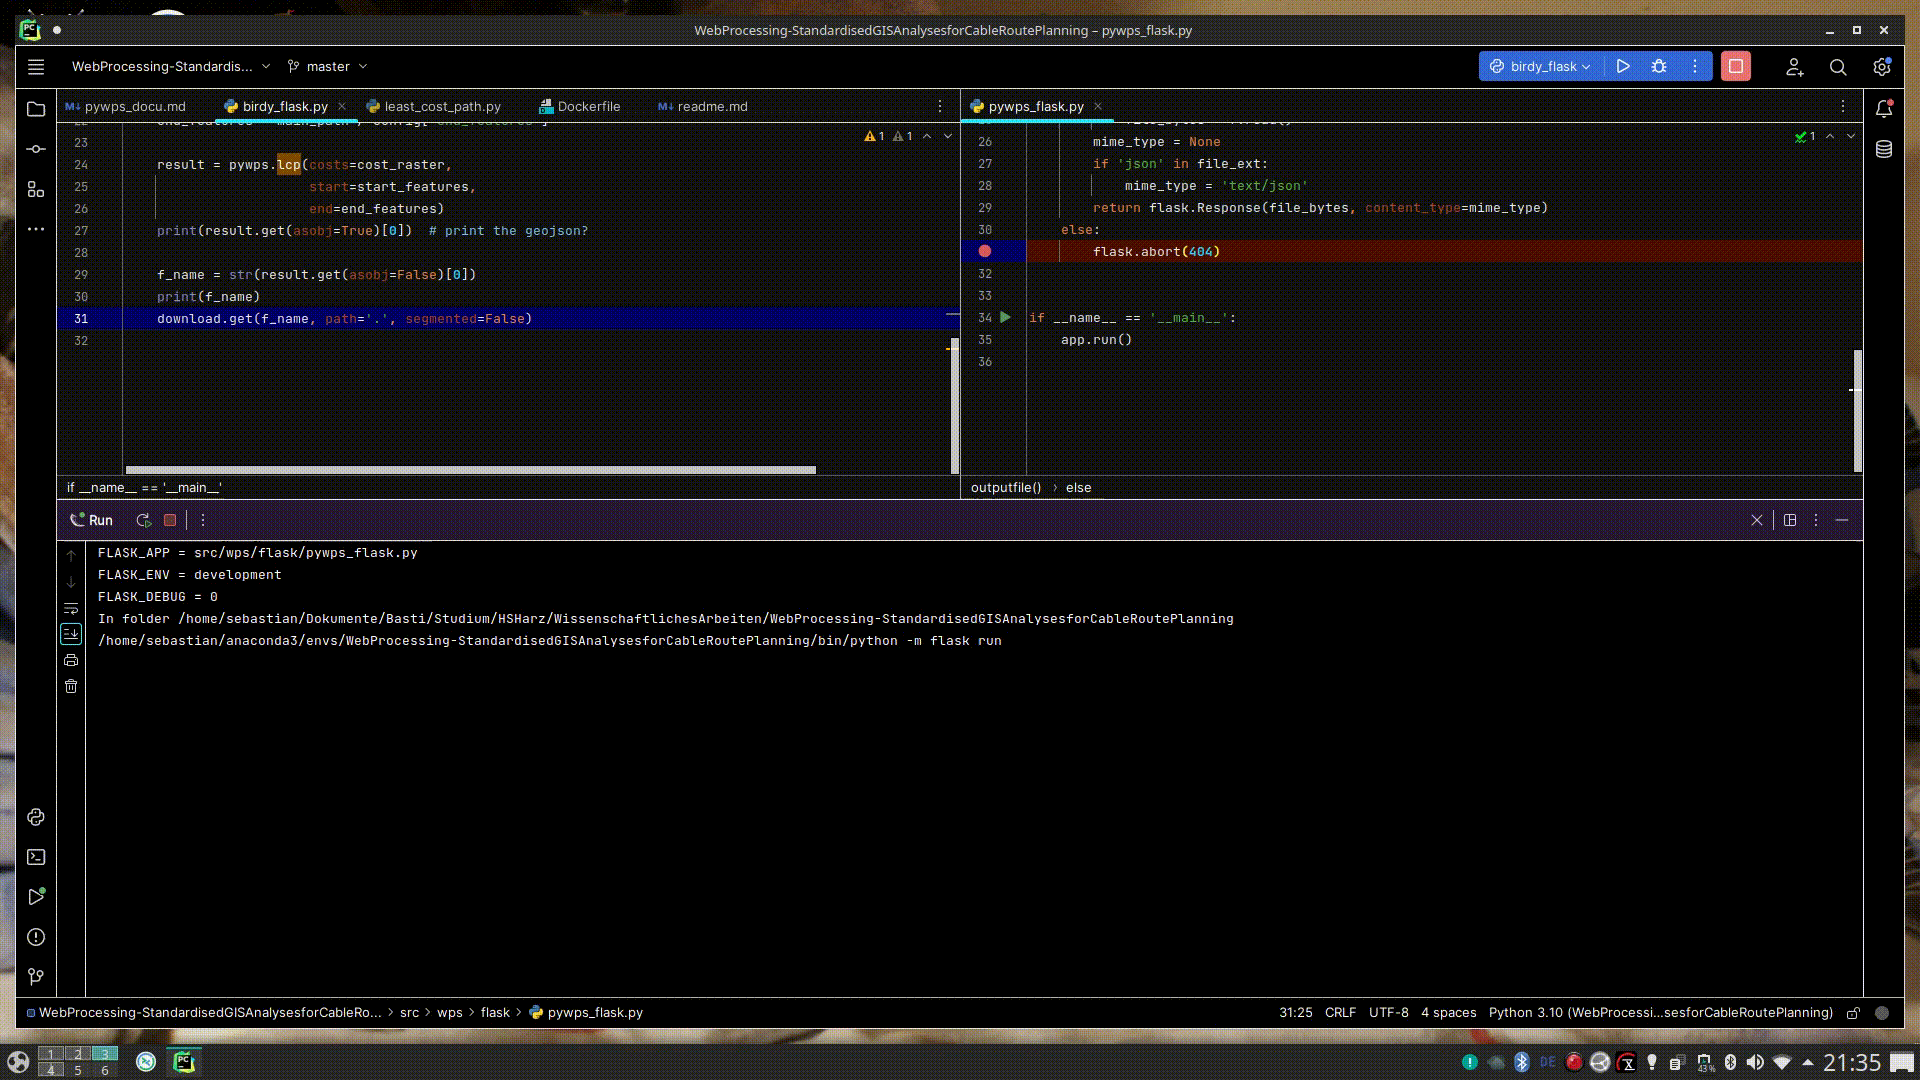
\includegraphics[width=0.75\textwidth]{images/wps.png}}{images/wps.gif}

	\end{frame}
	
	\section{From Cost Raster to Least Cost Path}
	\begin{frame}{Recap: Sampling Resolution}
		\begin{figure}
		\centering
		\subfloat[\centering 10~m]{{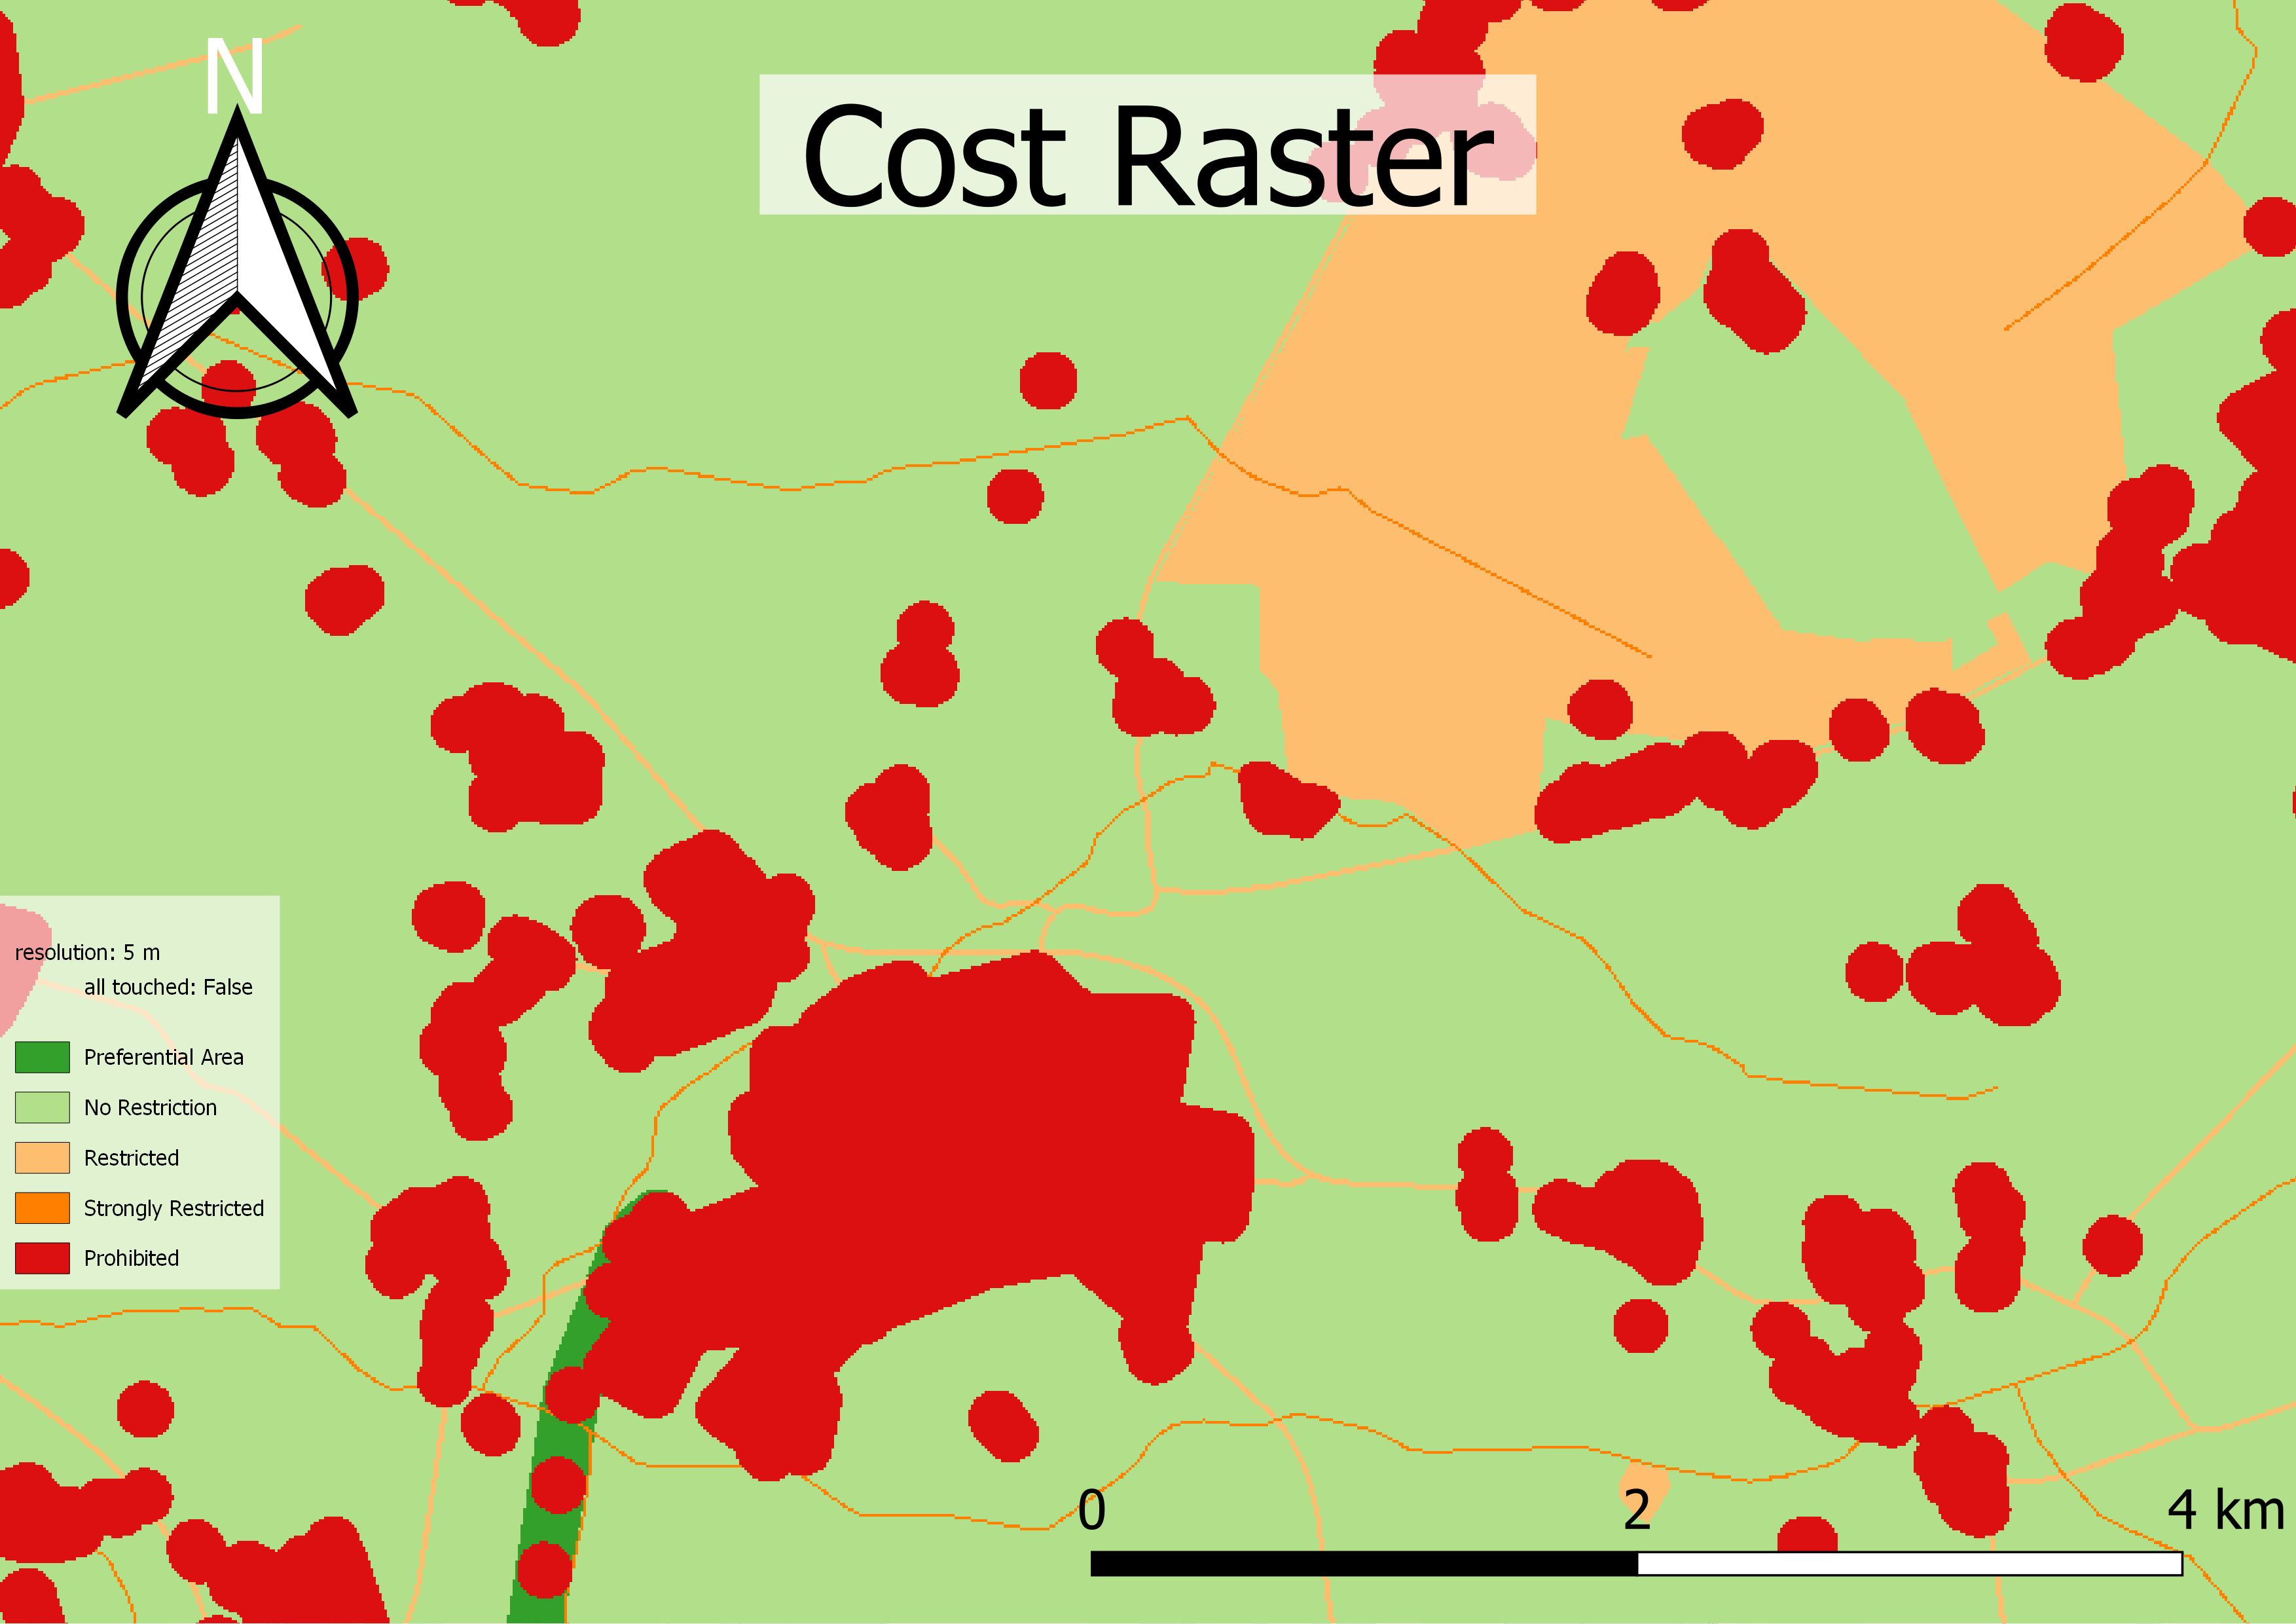
\includegraphics[width=.30\linewidth]{images/maps/CostRaster_10m_false.png} }}%
		\enskip
		\subfloat[\centering 25~m]{{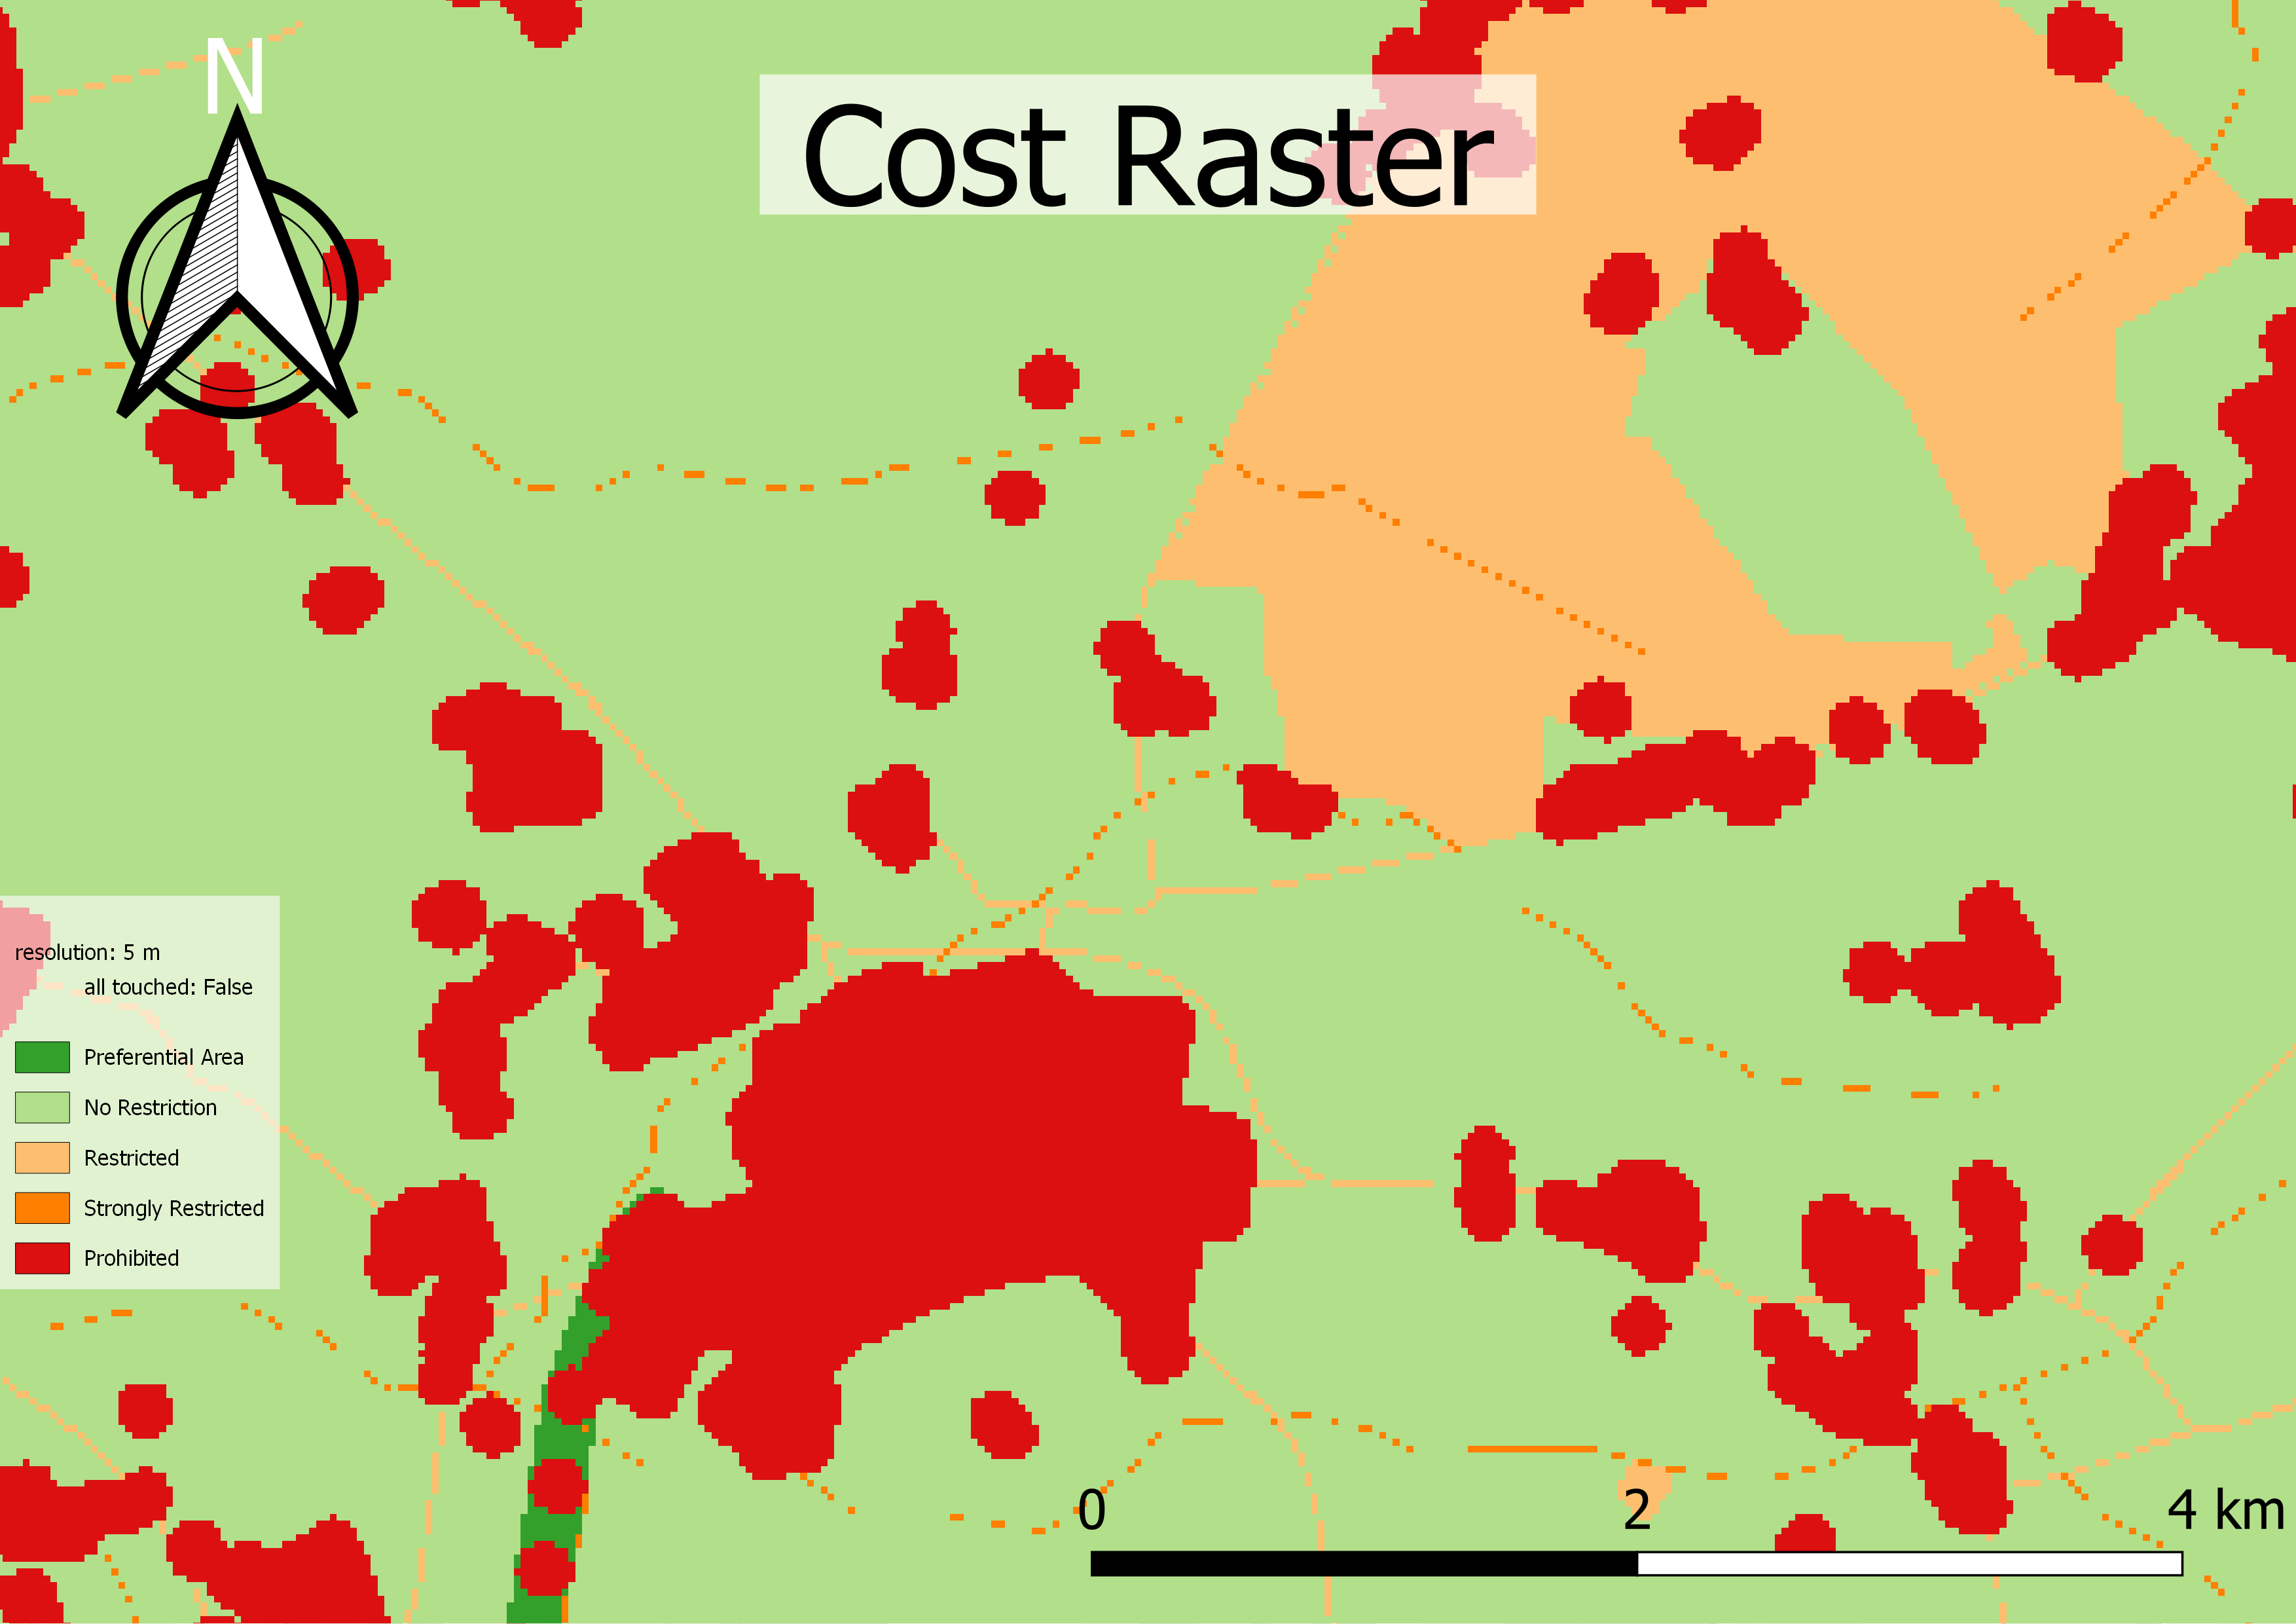
\includegraphics[width=.30\linewidth]{images/maps/CostRaster_25m_false.png} }}% 
		\enskip
		\subfloat[\centering 50~m]{{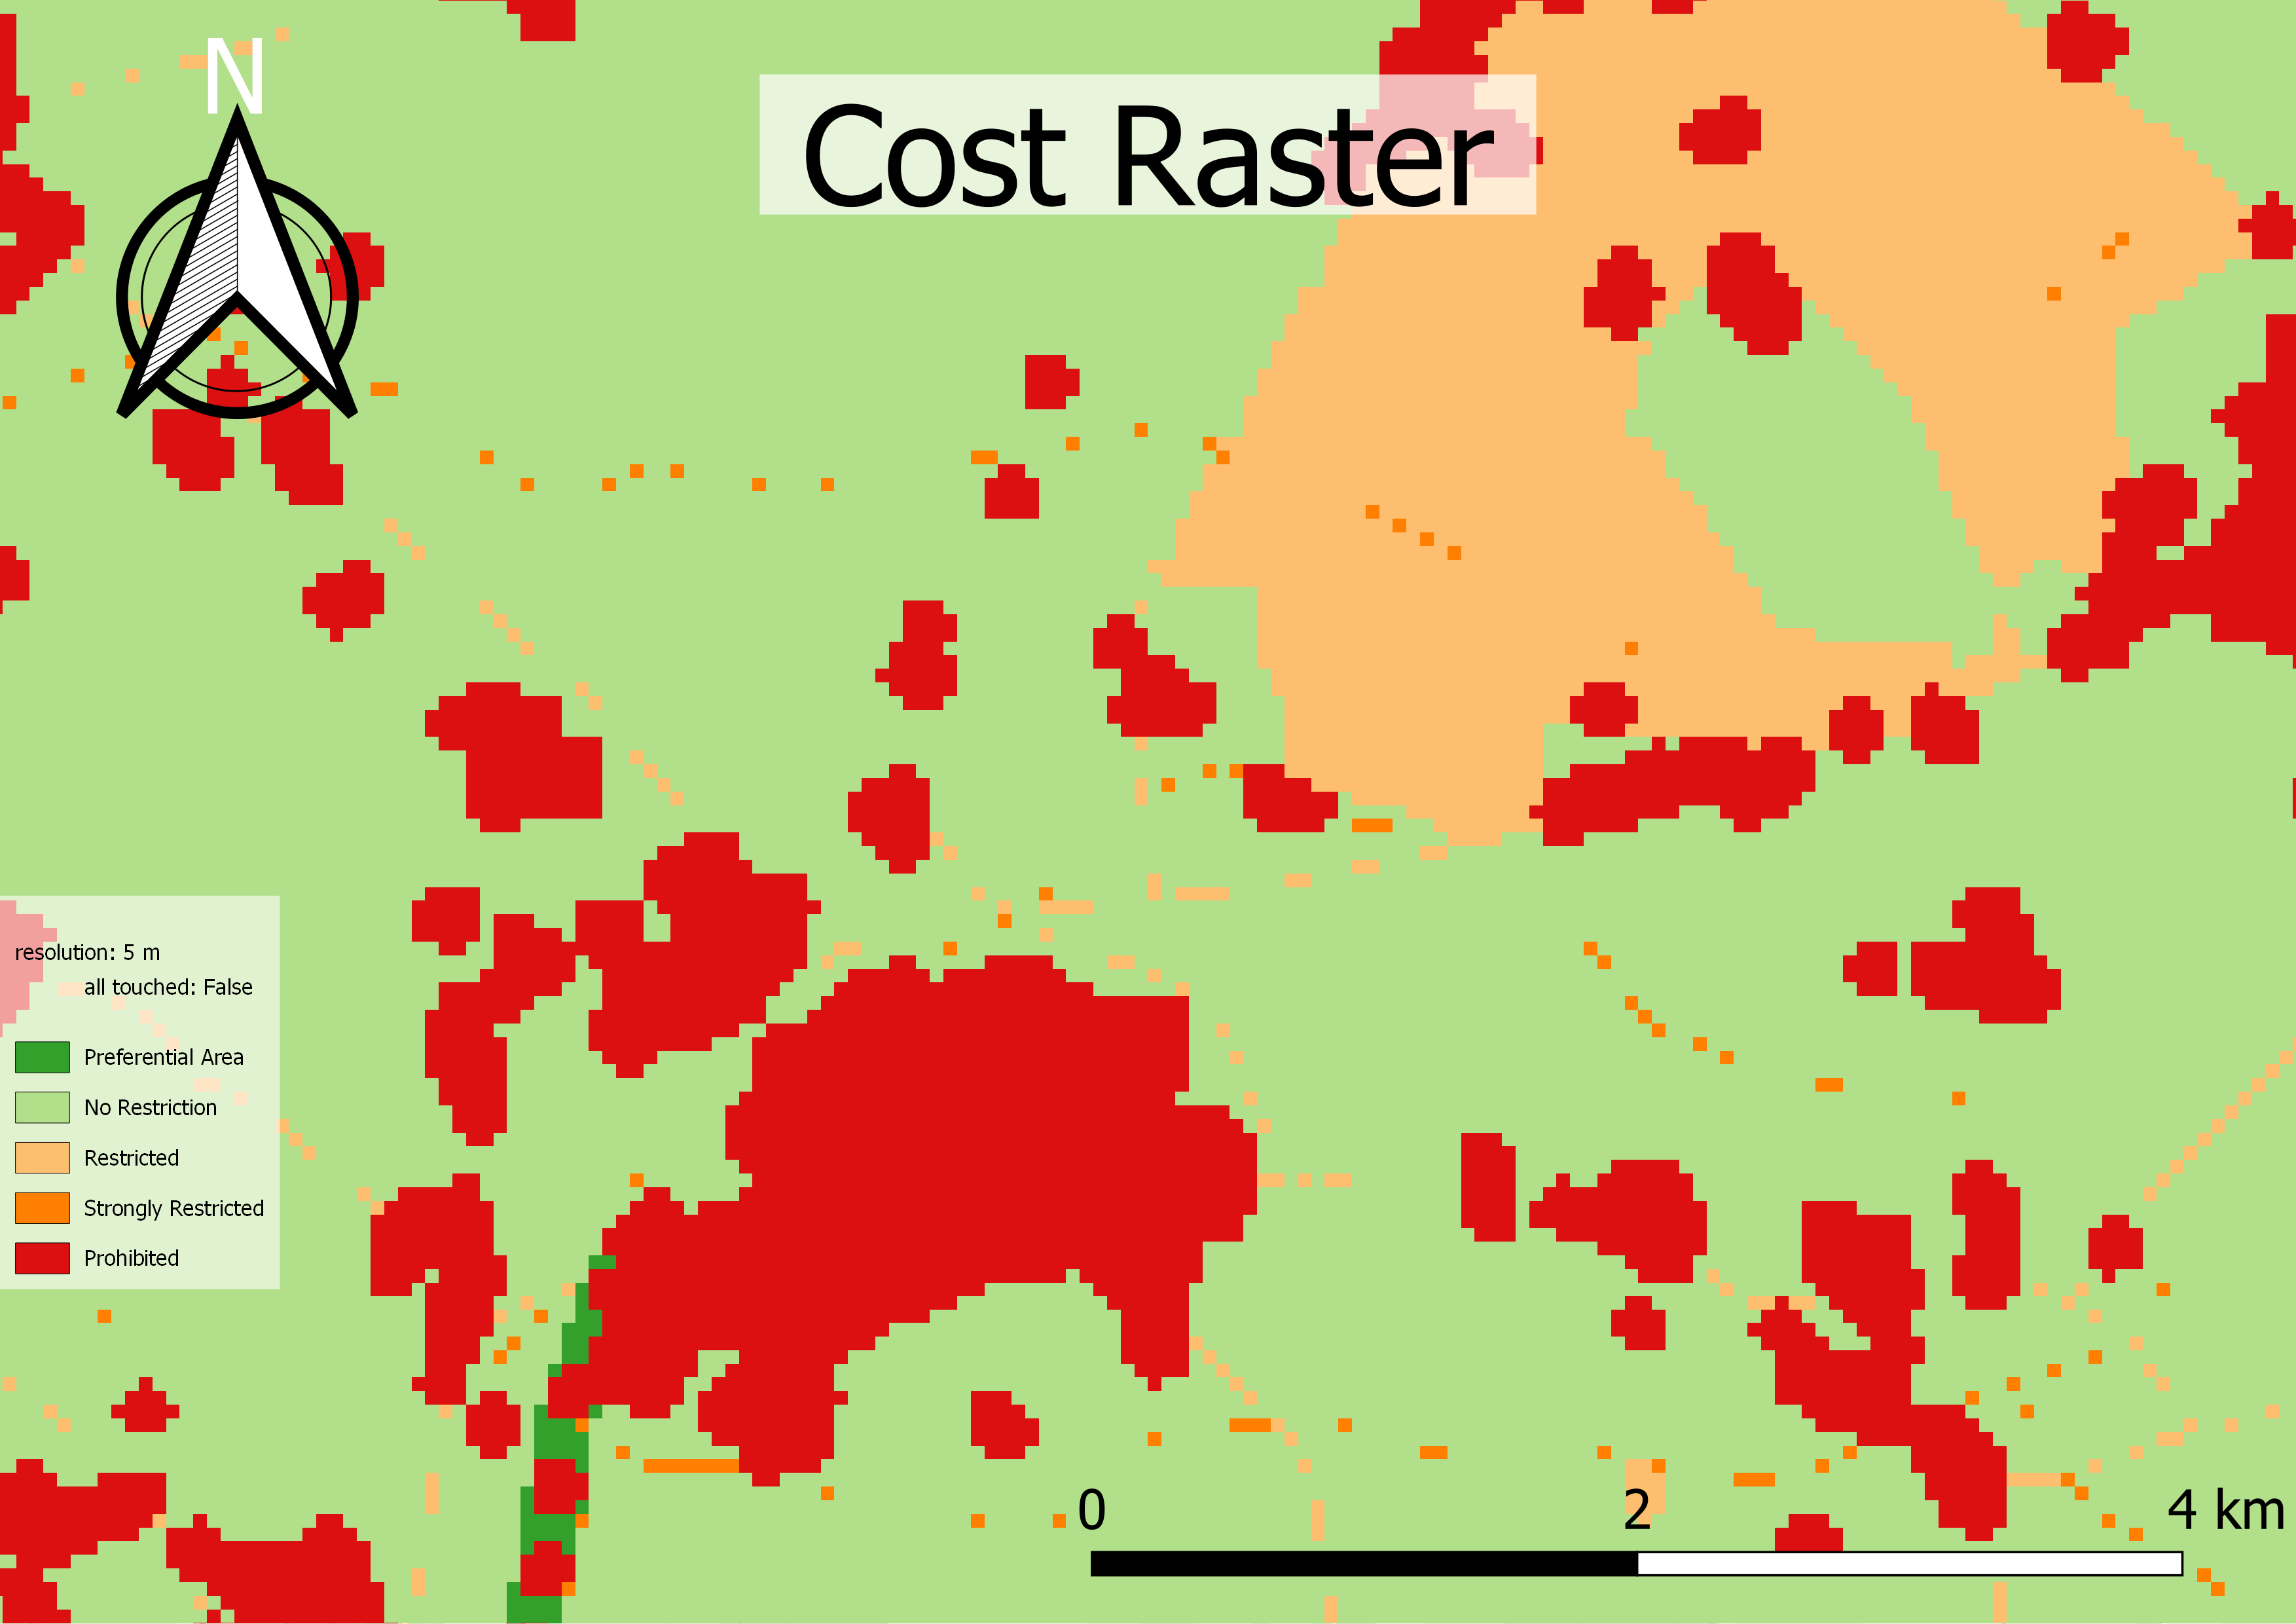
\includegraphics[width=.30\linewidth]{images/maps/CostRaster_50m_false.png} }}%
		
		\caption{Maps of the cost raster for all~touched set to False for different resolutions.}
		\label{fig:CostAllTouchedFalse}
		\end{figure}
	\end{frame}


	\begin{frame}{Recap: Sampling Resolution}
		\begin{figure}
		\begin{figure}
			\centering
			\subfloat[\centering 10~m]{{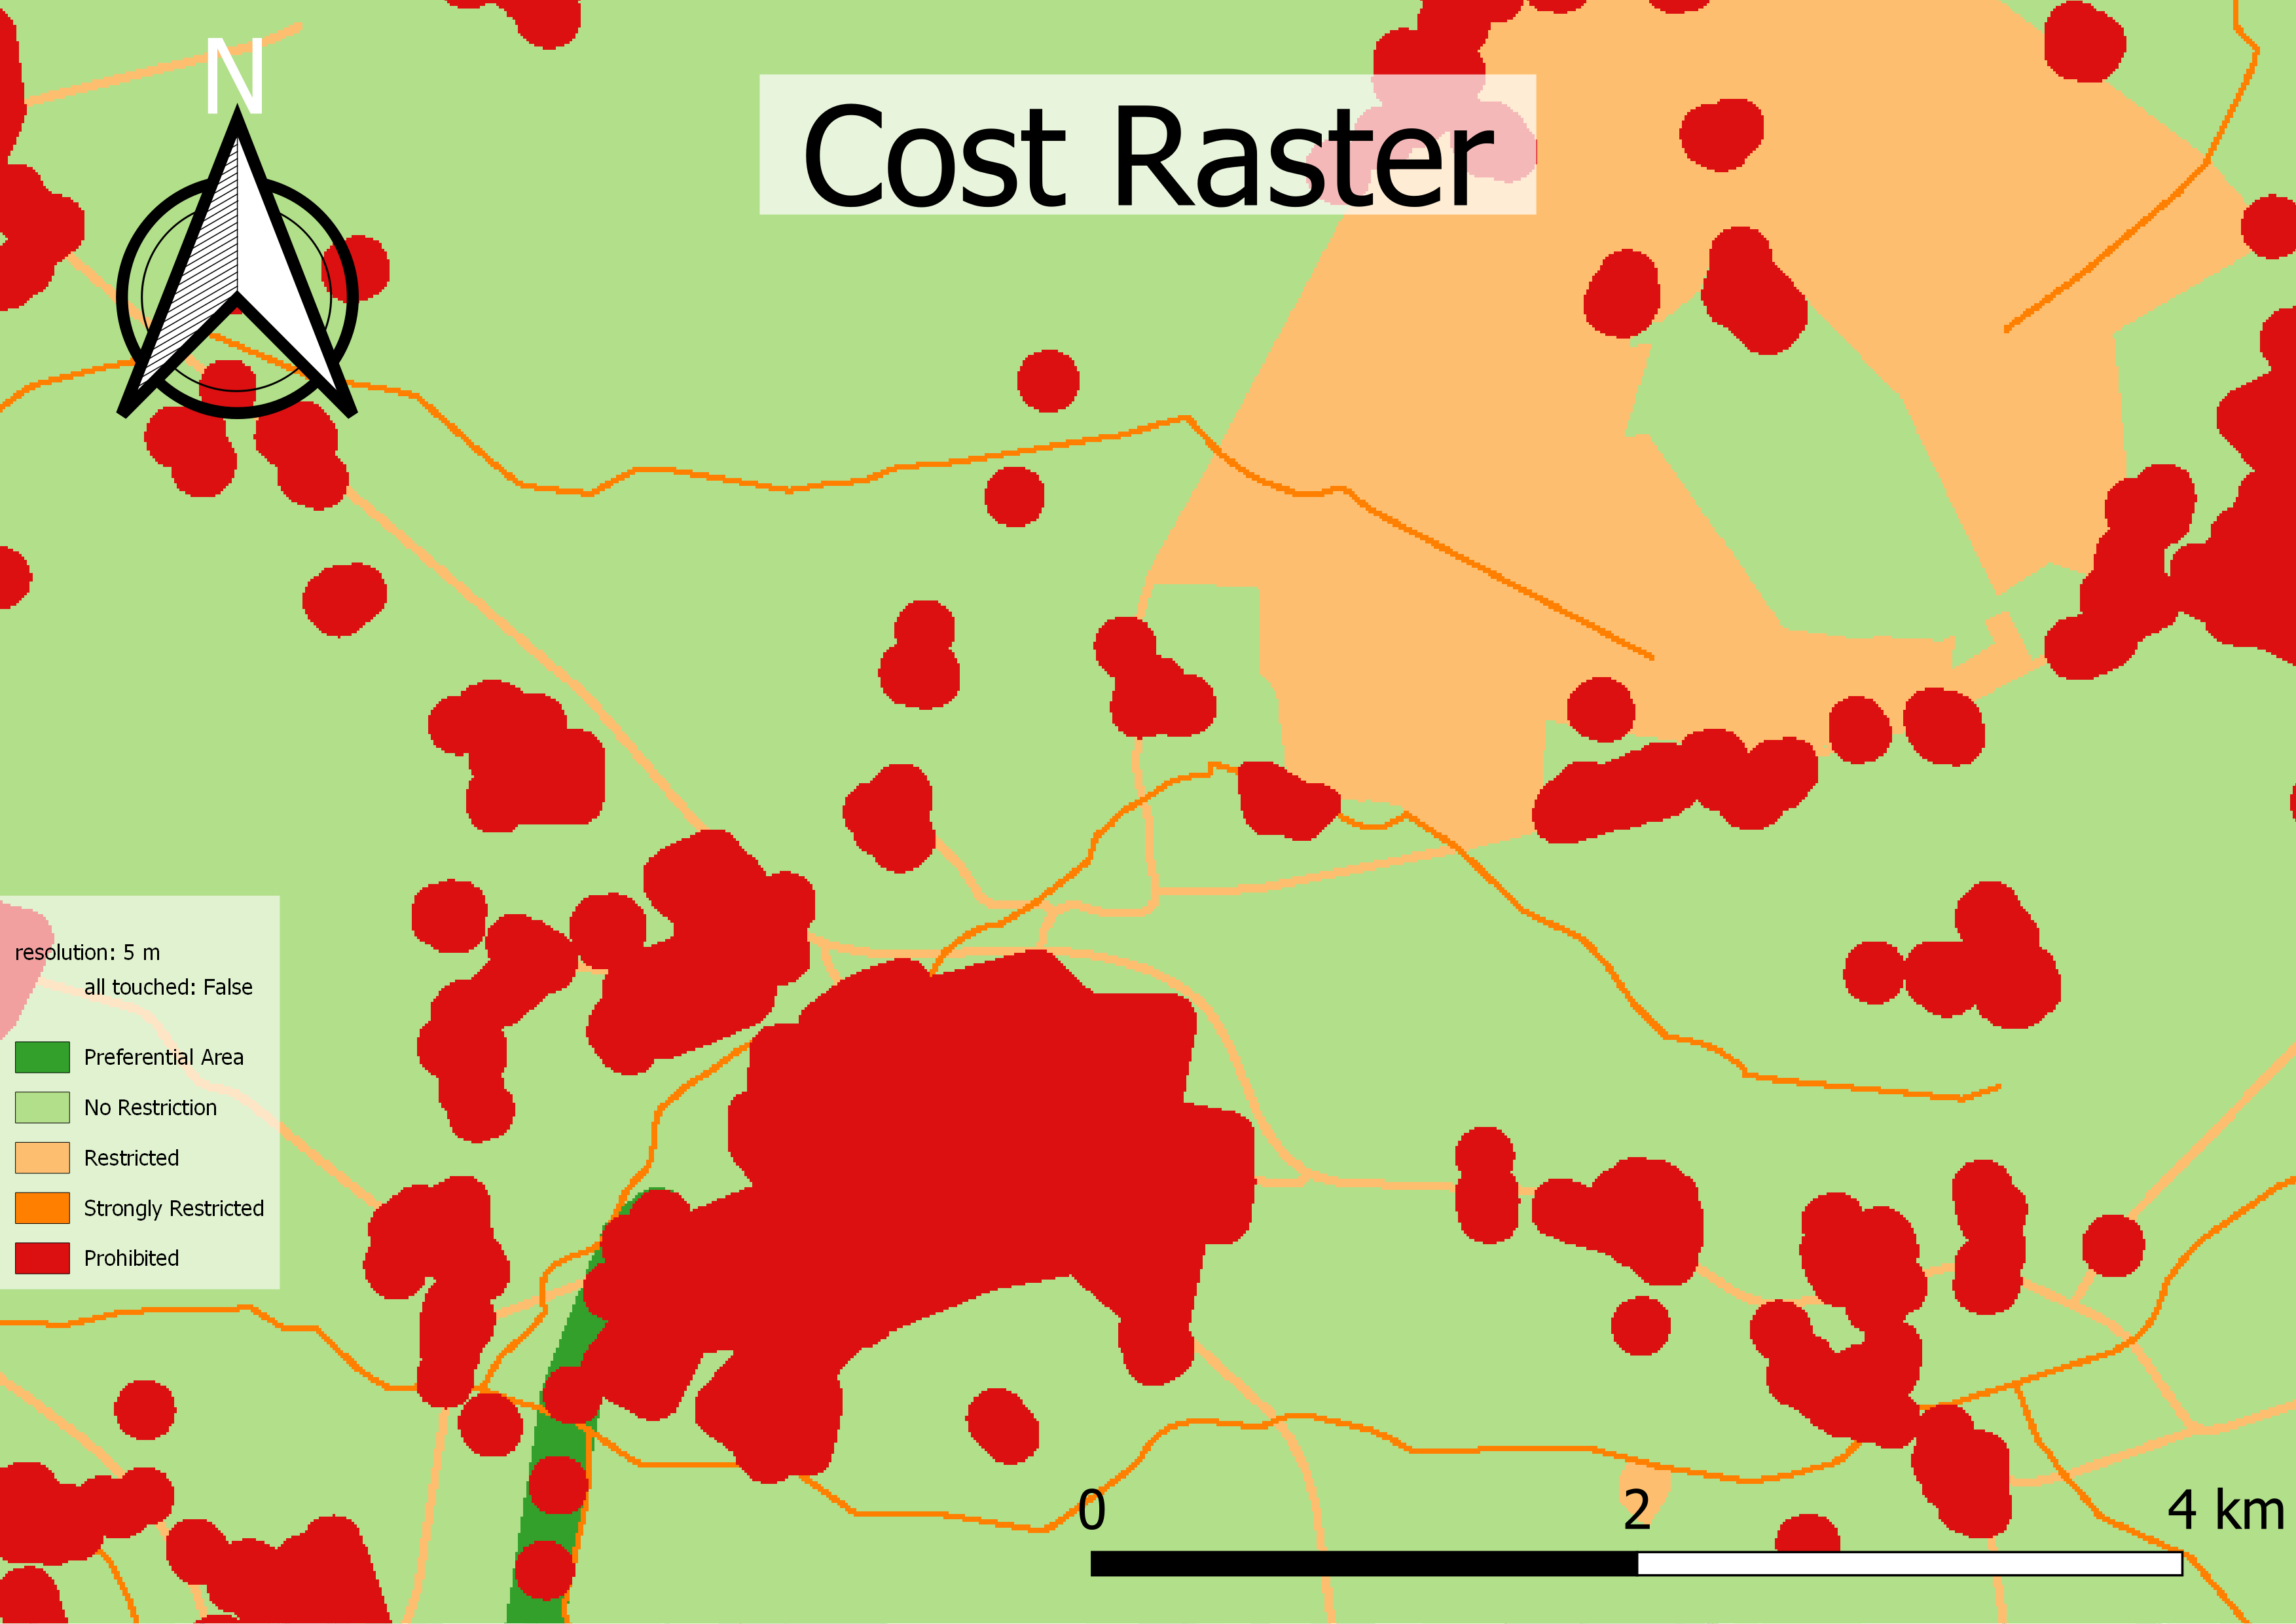
\includegraphics[width=.30\linewidth]{images/maps/CostRaster_10m_true.png} }}%
			\enskip
			\subfloat[\centering 25~m]{{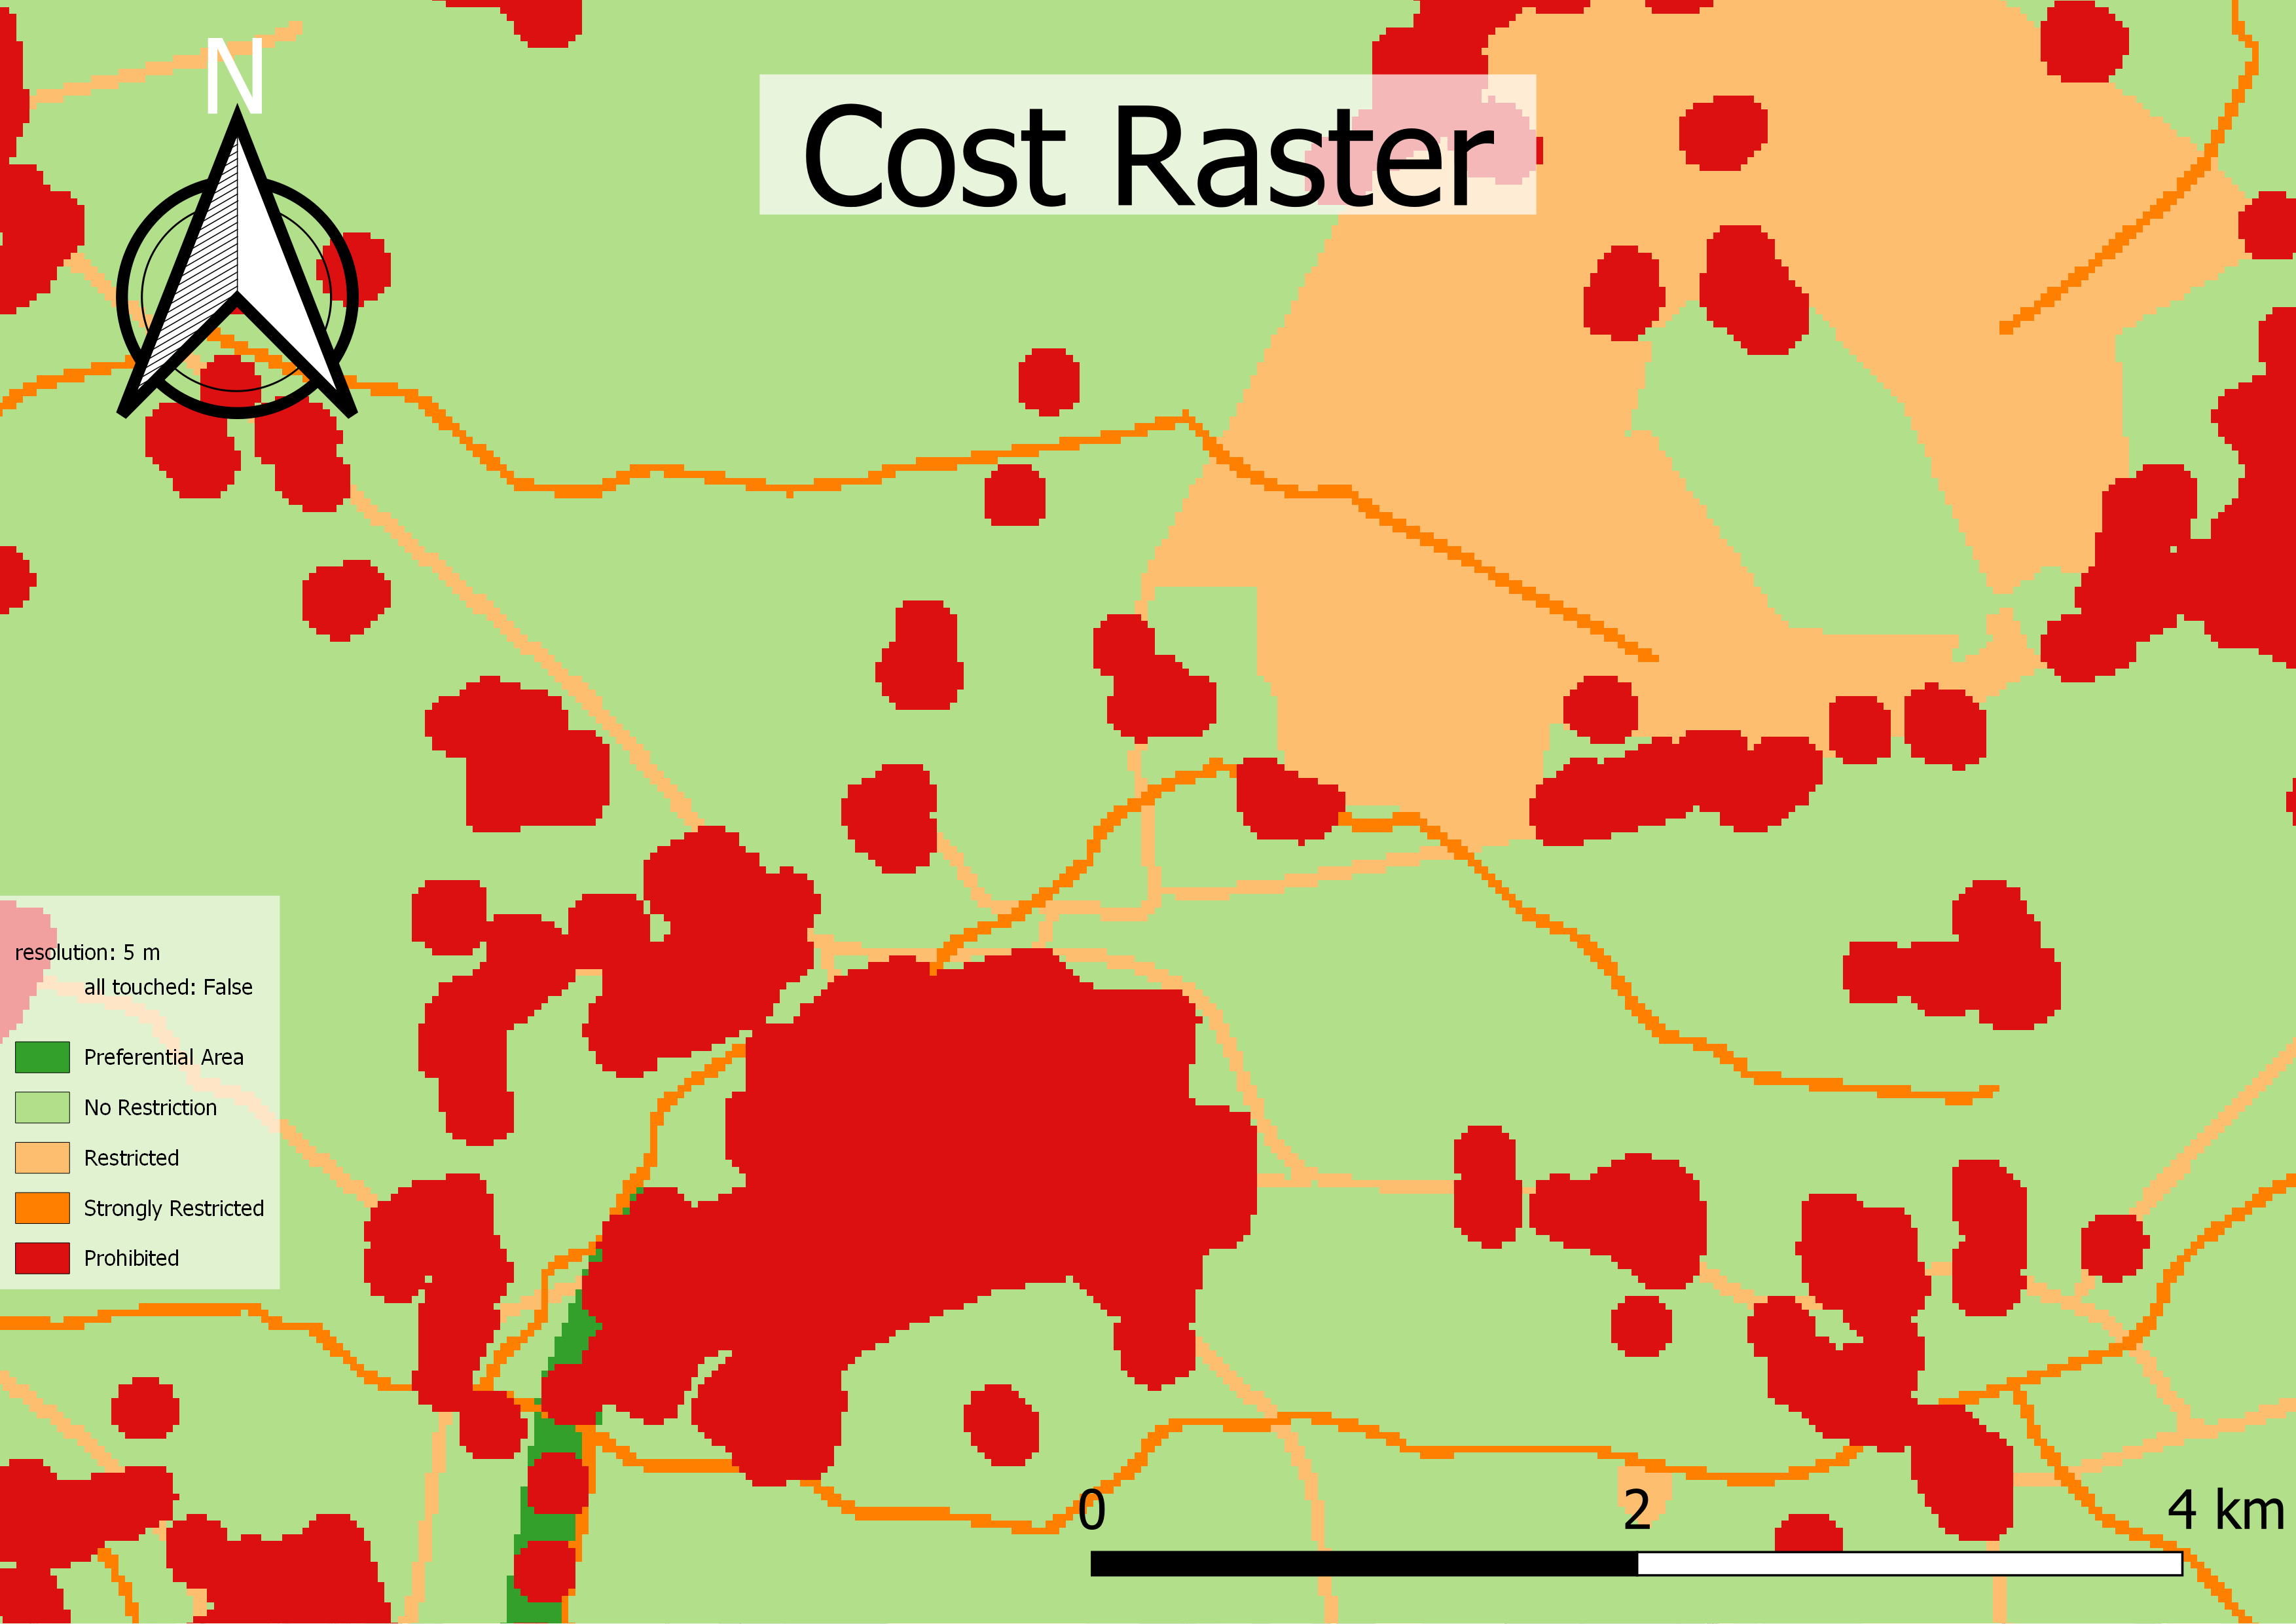
\includegraphics[width=.30\linewidth]{images/maps/CostRaster_25m_true.png} }}% 
			\enskip
			\subfloat[\centering 50~m]{{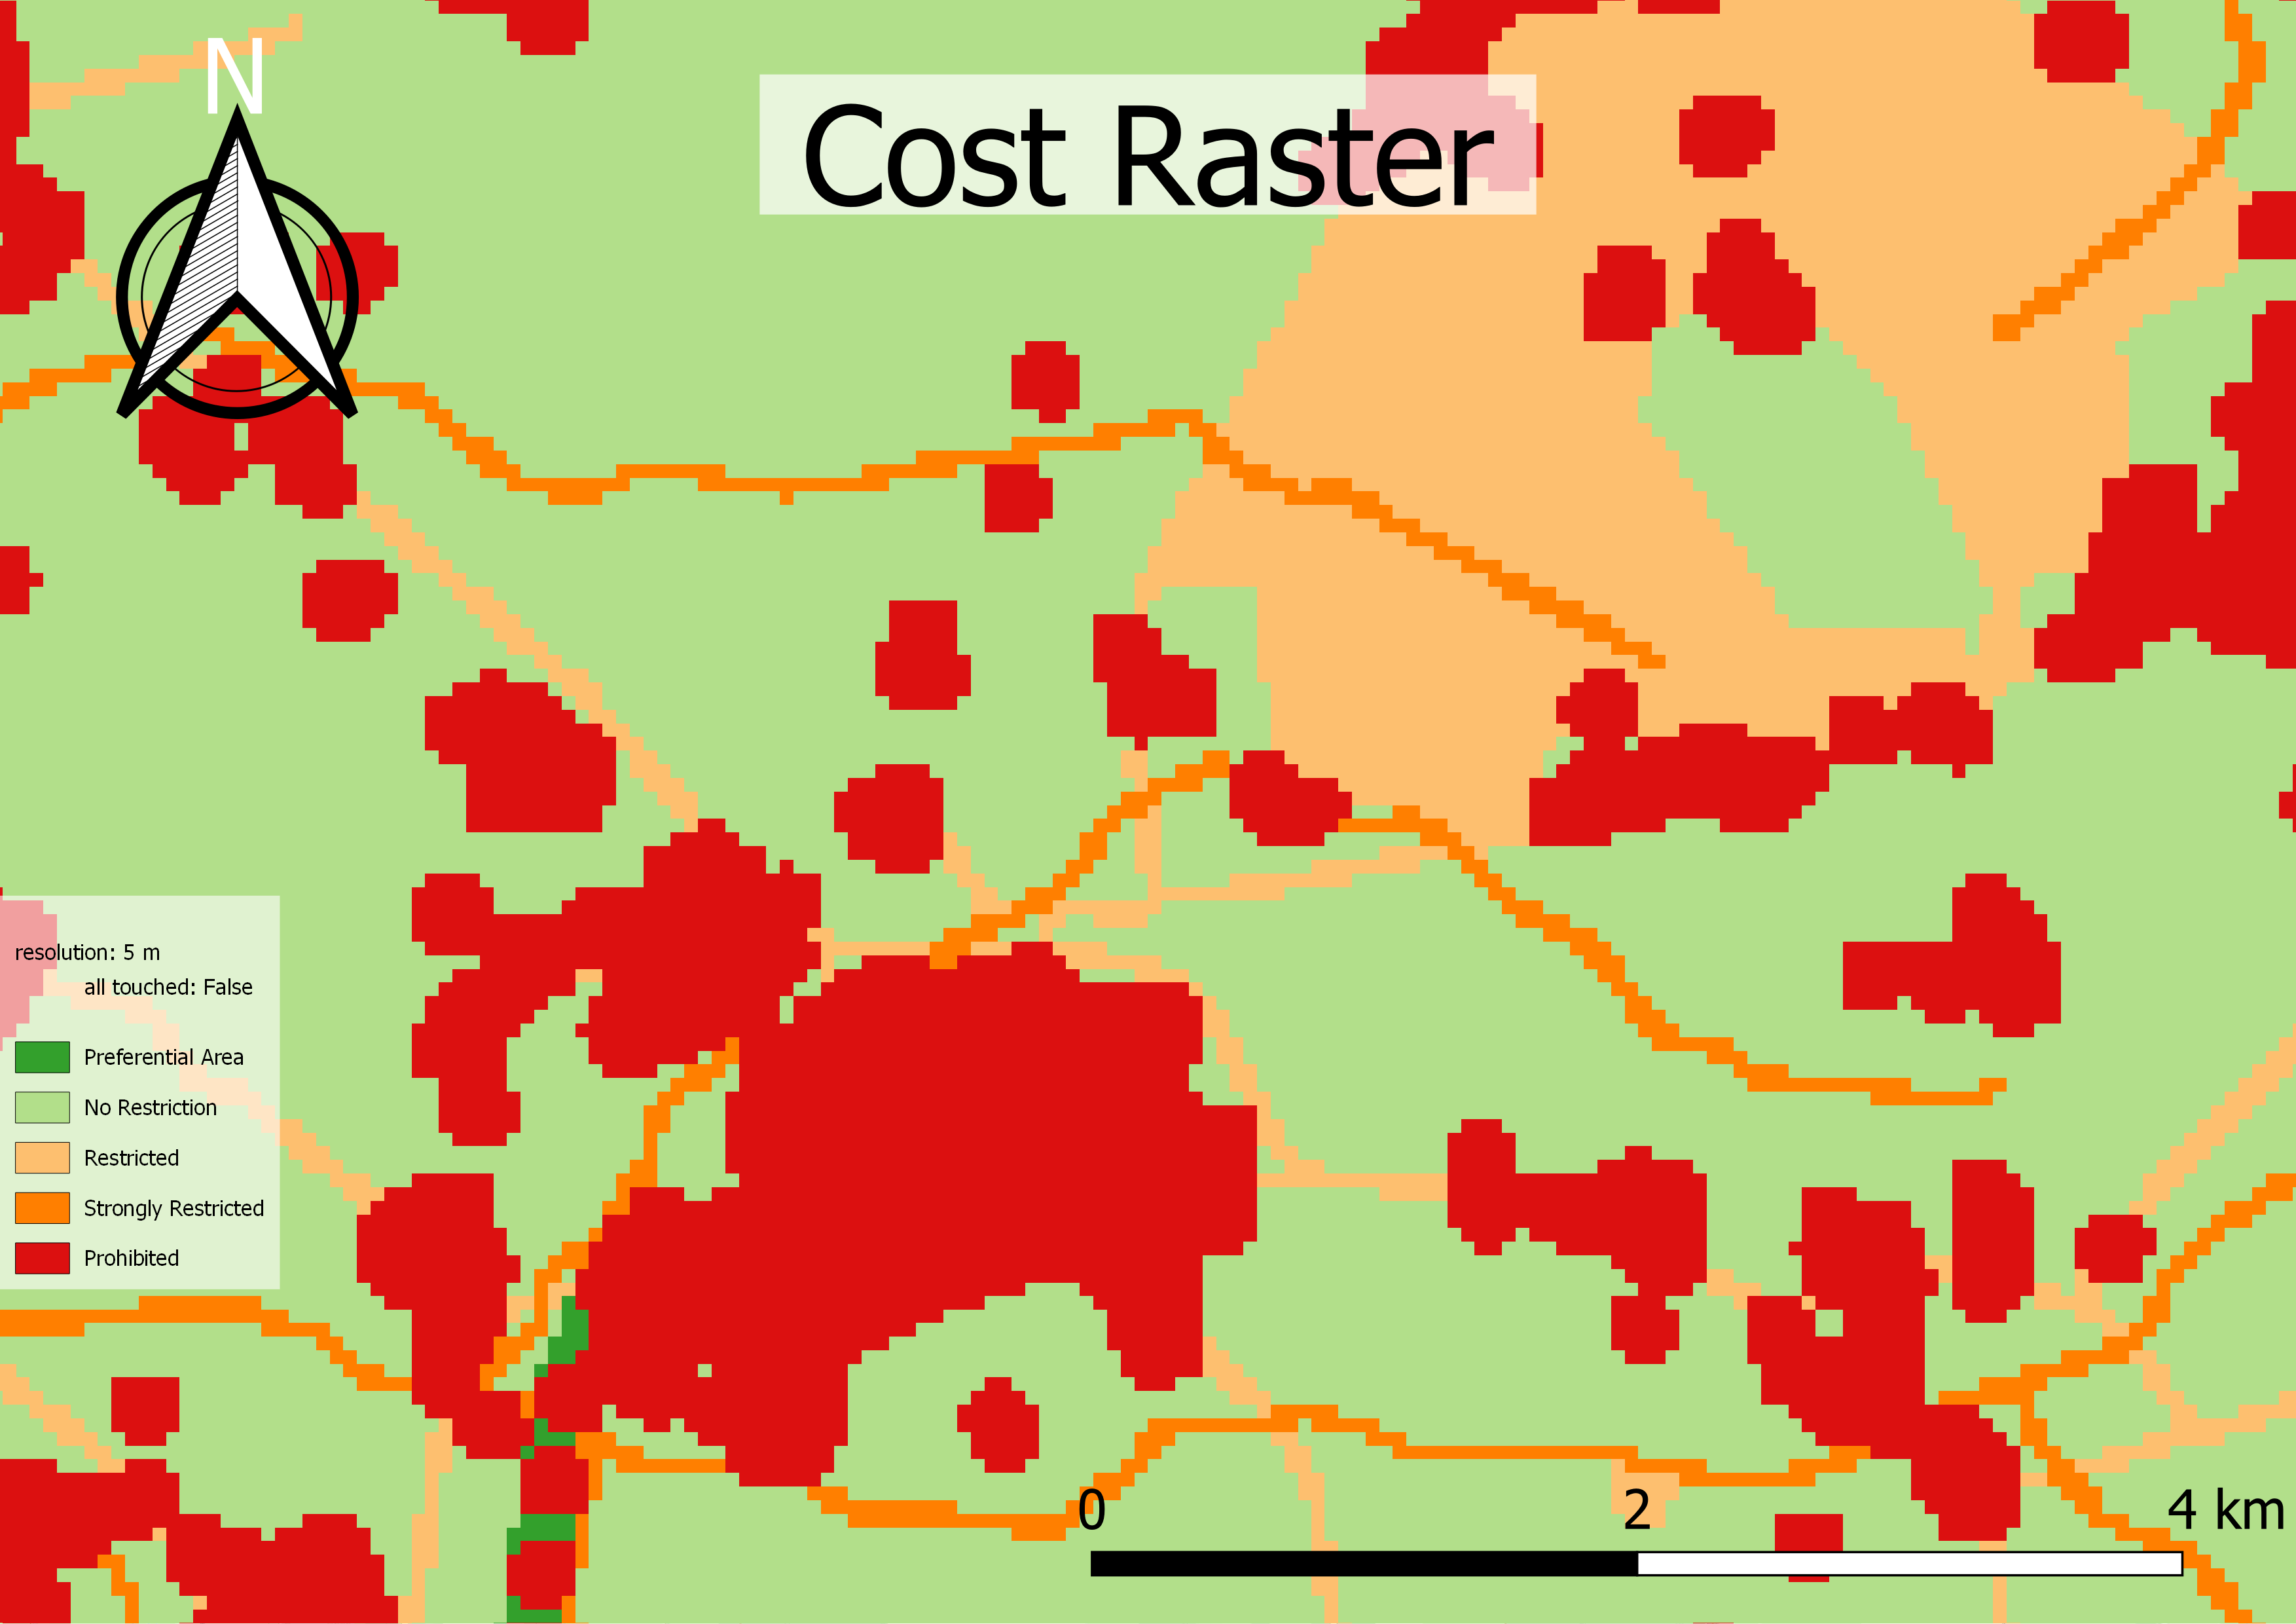
\includegraphics[width=.30\linewidth]{images/maps/CostRaster_50m_true.png} }}%
			
			\caption{Maps of the cost raster for all~touched set to True for different resolutions.}
			\label{fig:CostAllTouchedTrue}
		\end{figure}
		\end{figure}
	\end{frame}

	
	
	\begin{frame}{From Cost Raster to Least Cost Path}
		\begin{figure}
			\centering
			\subfloat[\centering Cost Raster.]{{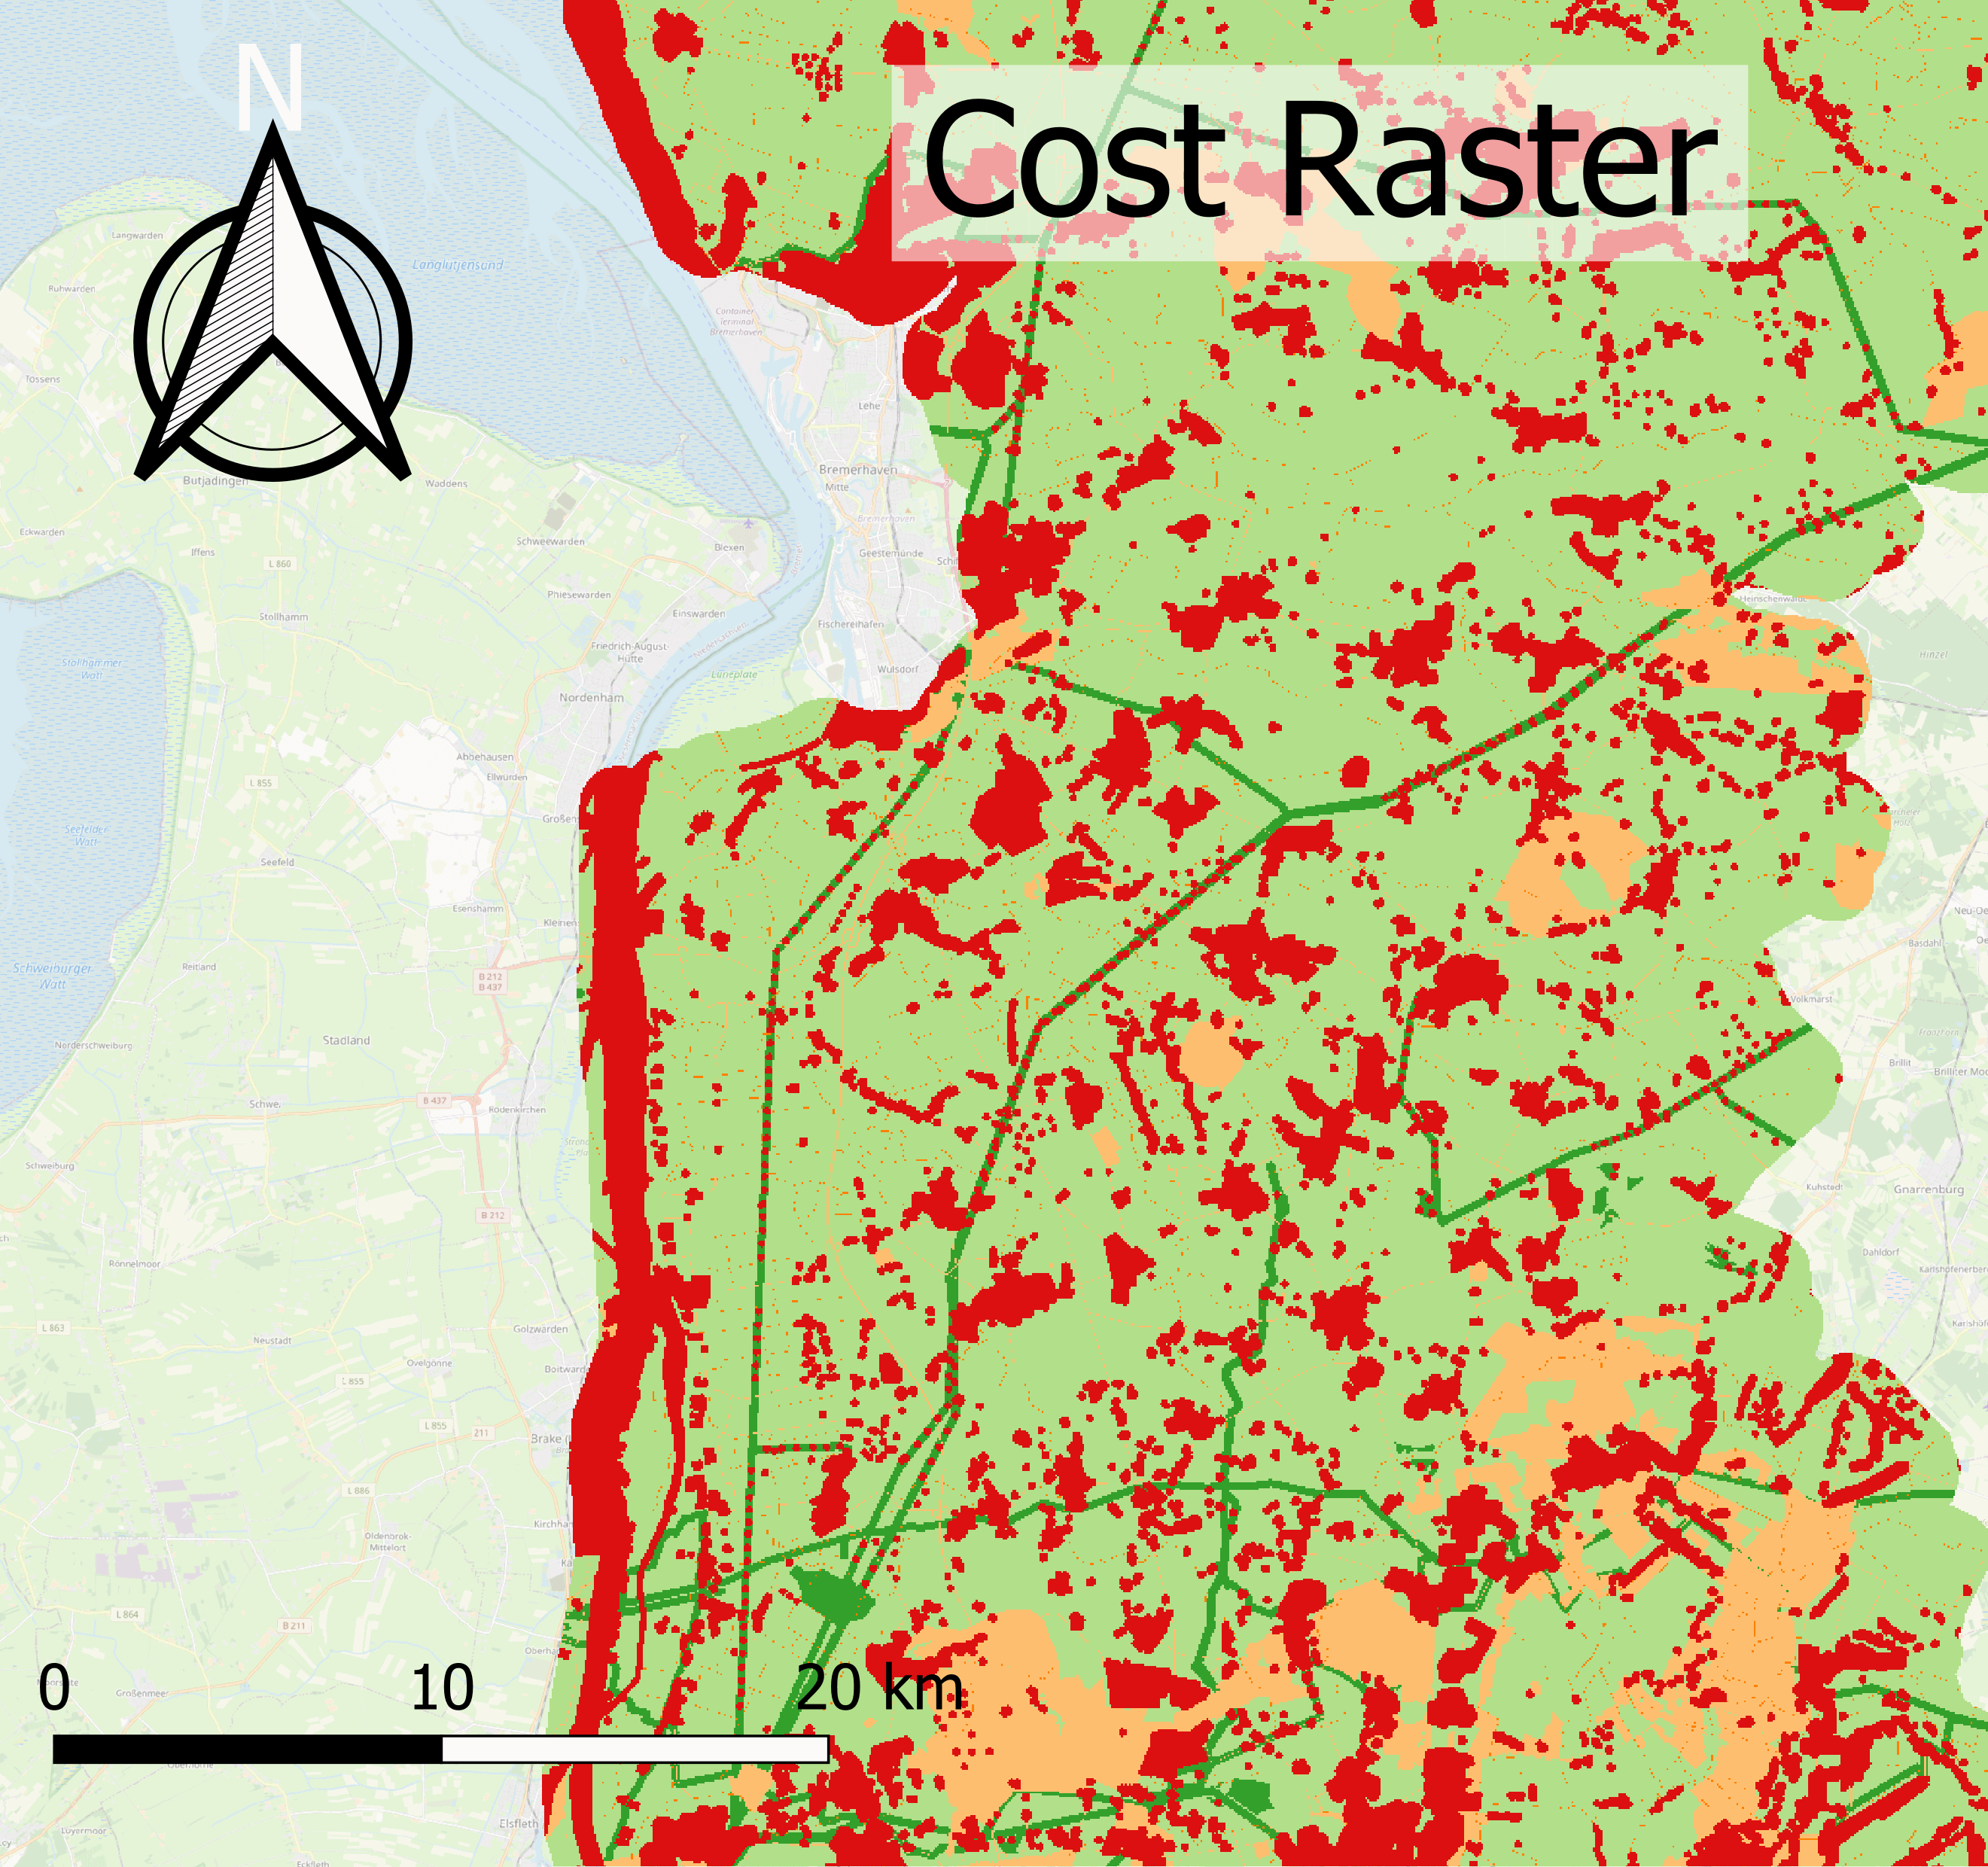
\includegraphics[width=.30\linewidth]{images/maps/CostRasterExample_cut.png} }}%
			\enskip
			\subfloat[\centering Aggregated Cost Raster.]{{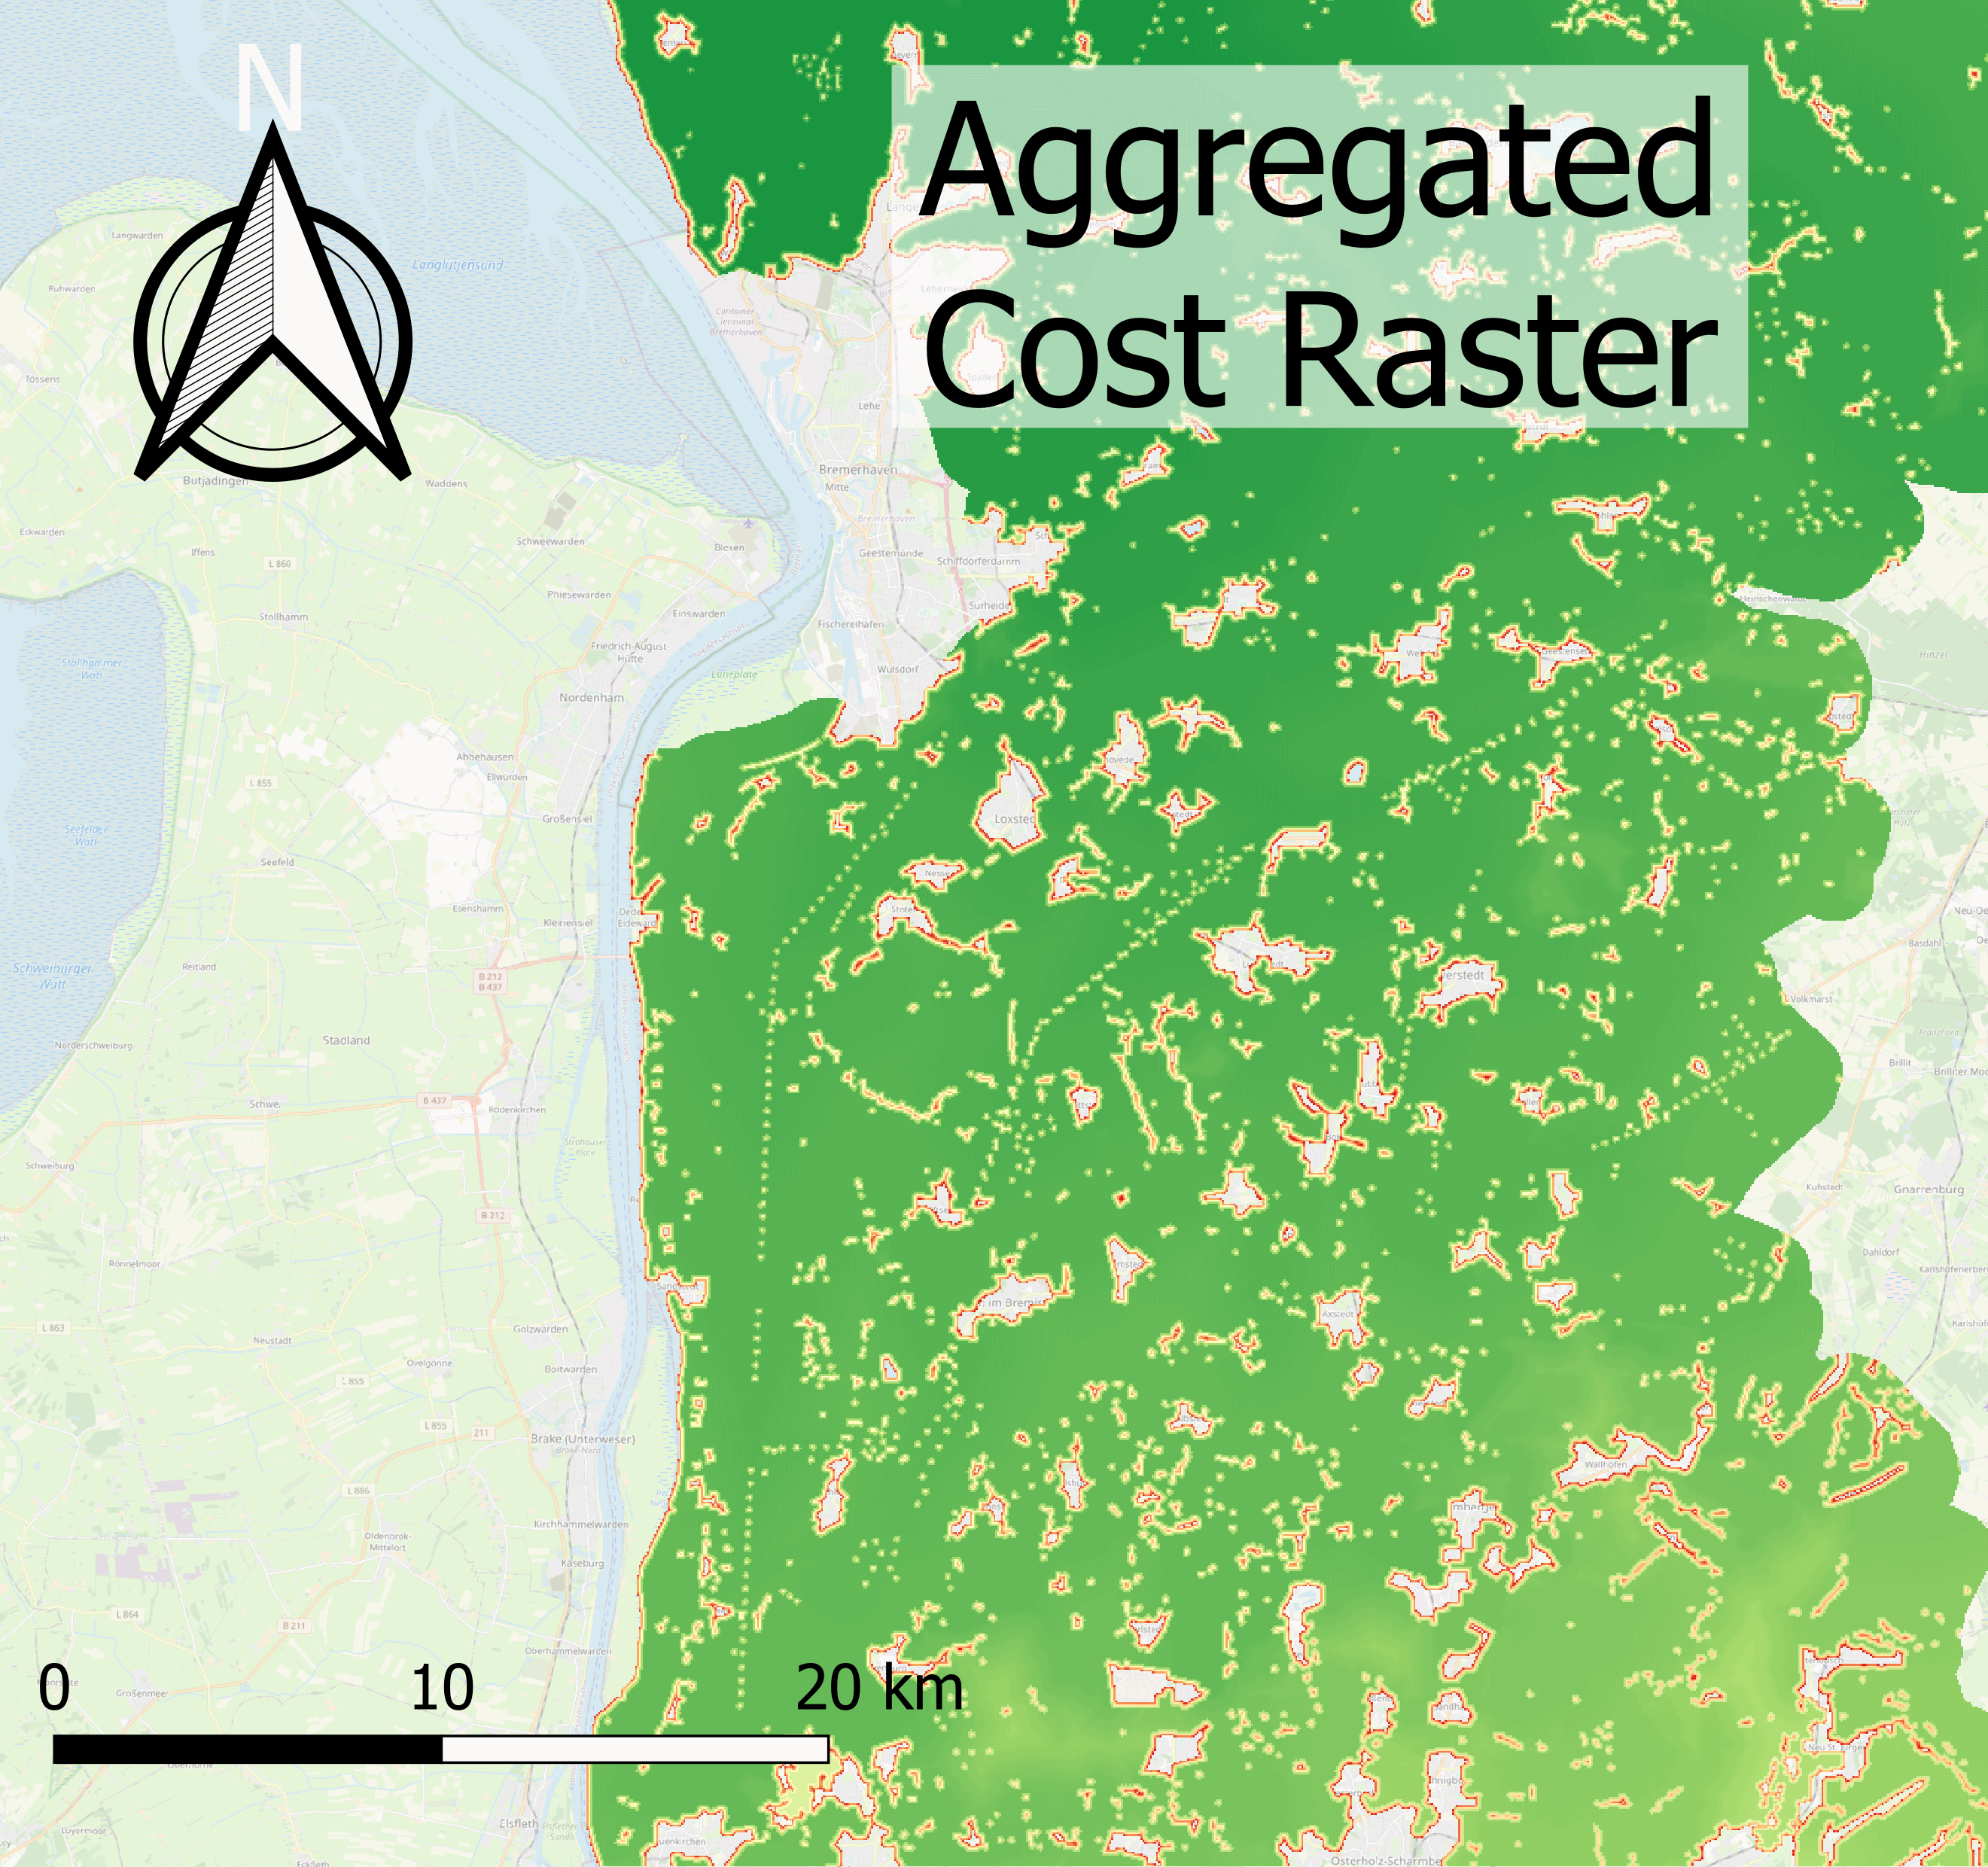
\includegraphics[width=.30\linewidth]{images/maps/AggregatedCosts_cut.png} \label{fig:aggregation}}}%
			\enskip
			\subfloat[\centering Least Cost Path.]{{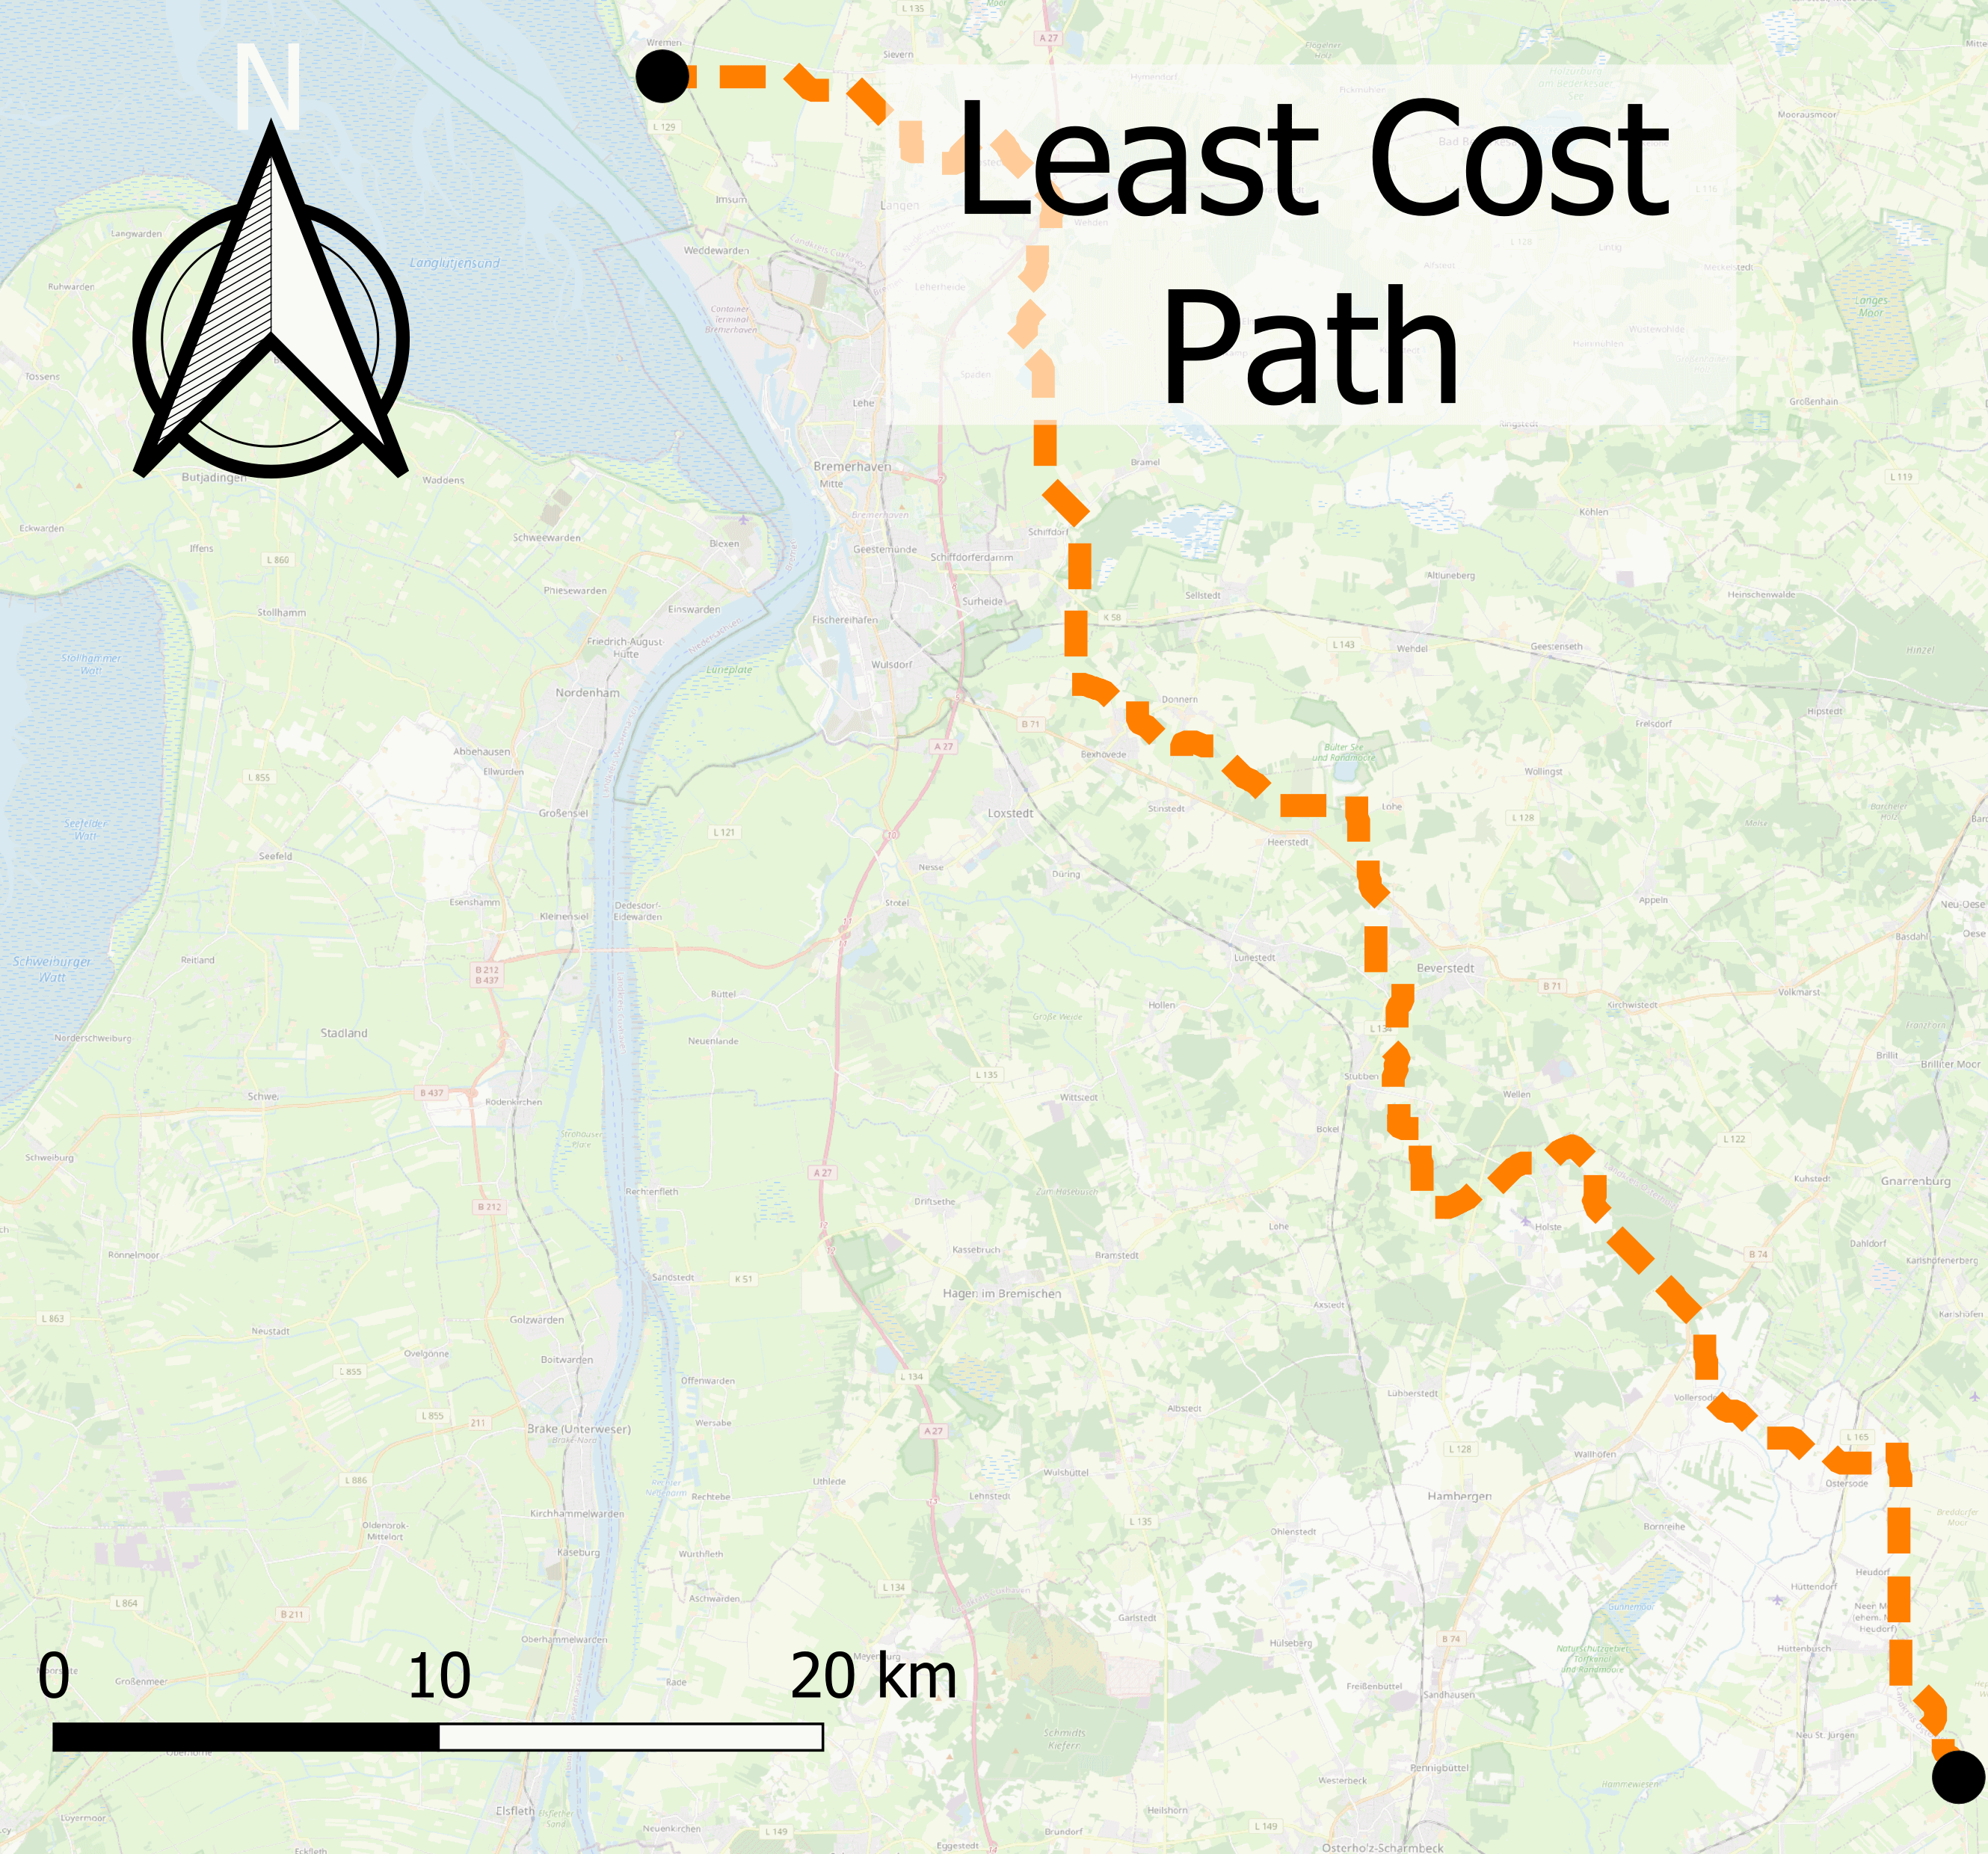
\includegraphics[width=.30\linewidth]{images/maps/LeastCostPathExample_cut.png} }}%
			
			\caption{Figures of the different steps for the Least Cost Path generation for a resolution of 50~m, all~touched set to False.}
			\label{fig:costs2path}
		\end{figure}
	\end{frame}
	
	\section{Comparing Paths}
	\begin{frame}{Comparing: Map}
		\begin{figure}
			\centering
			
			\subfloat[\centering all touched False.]{{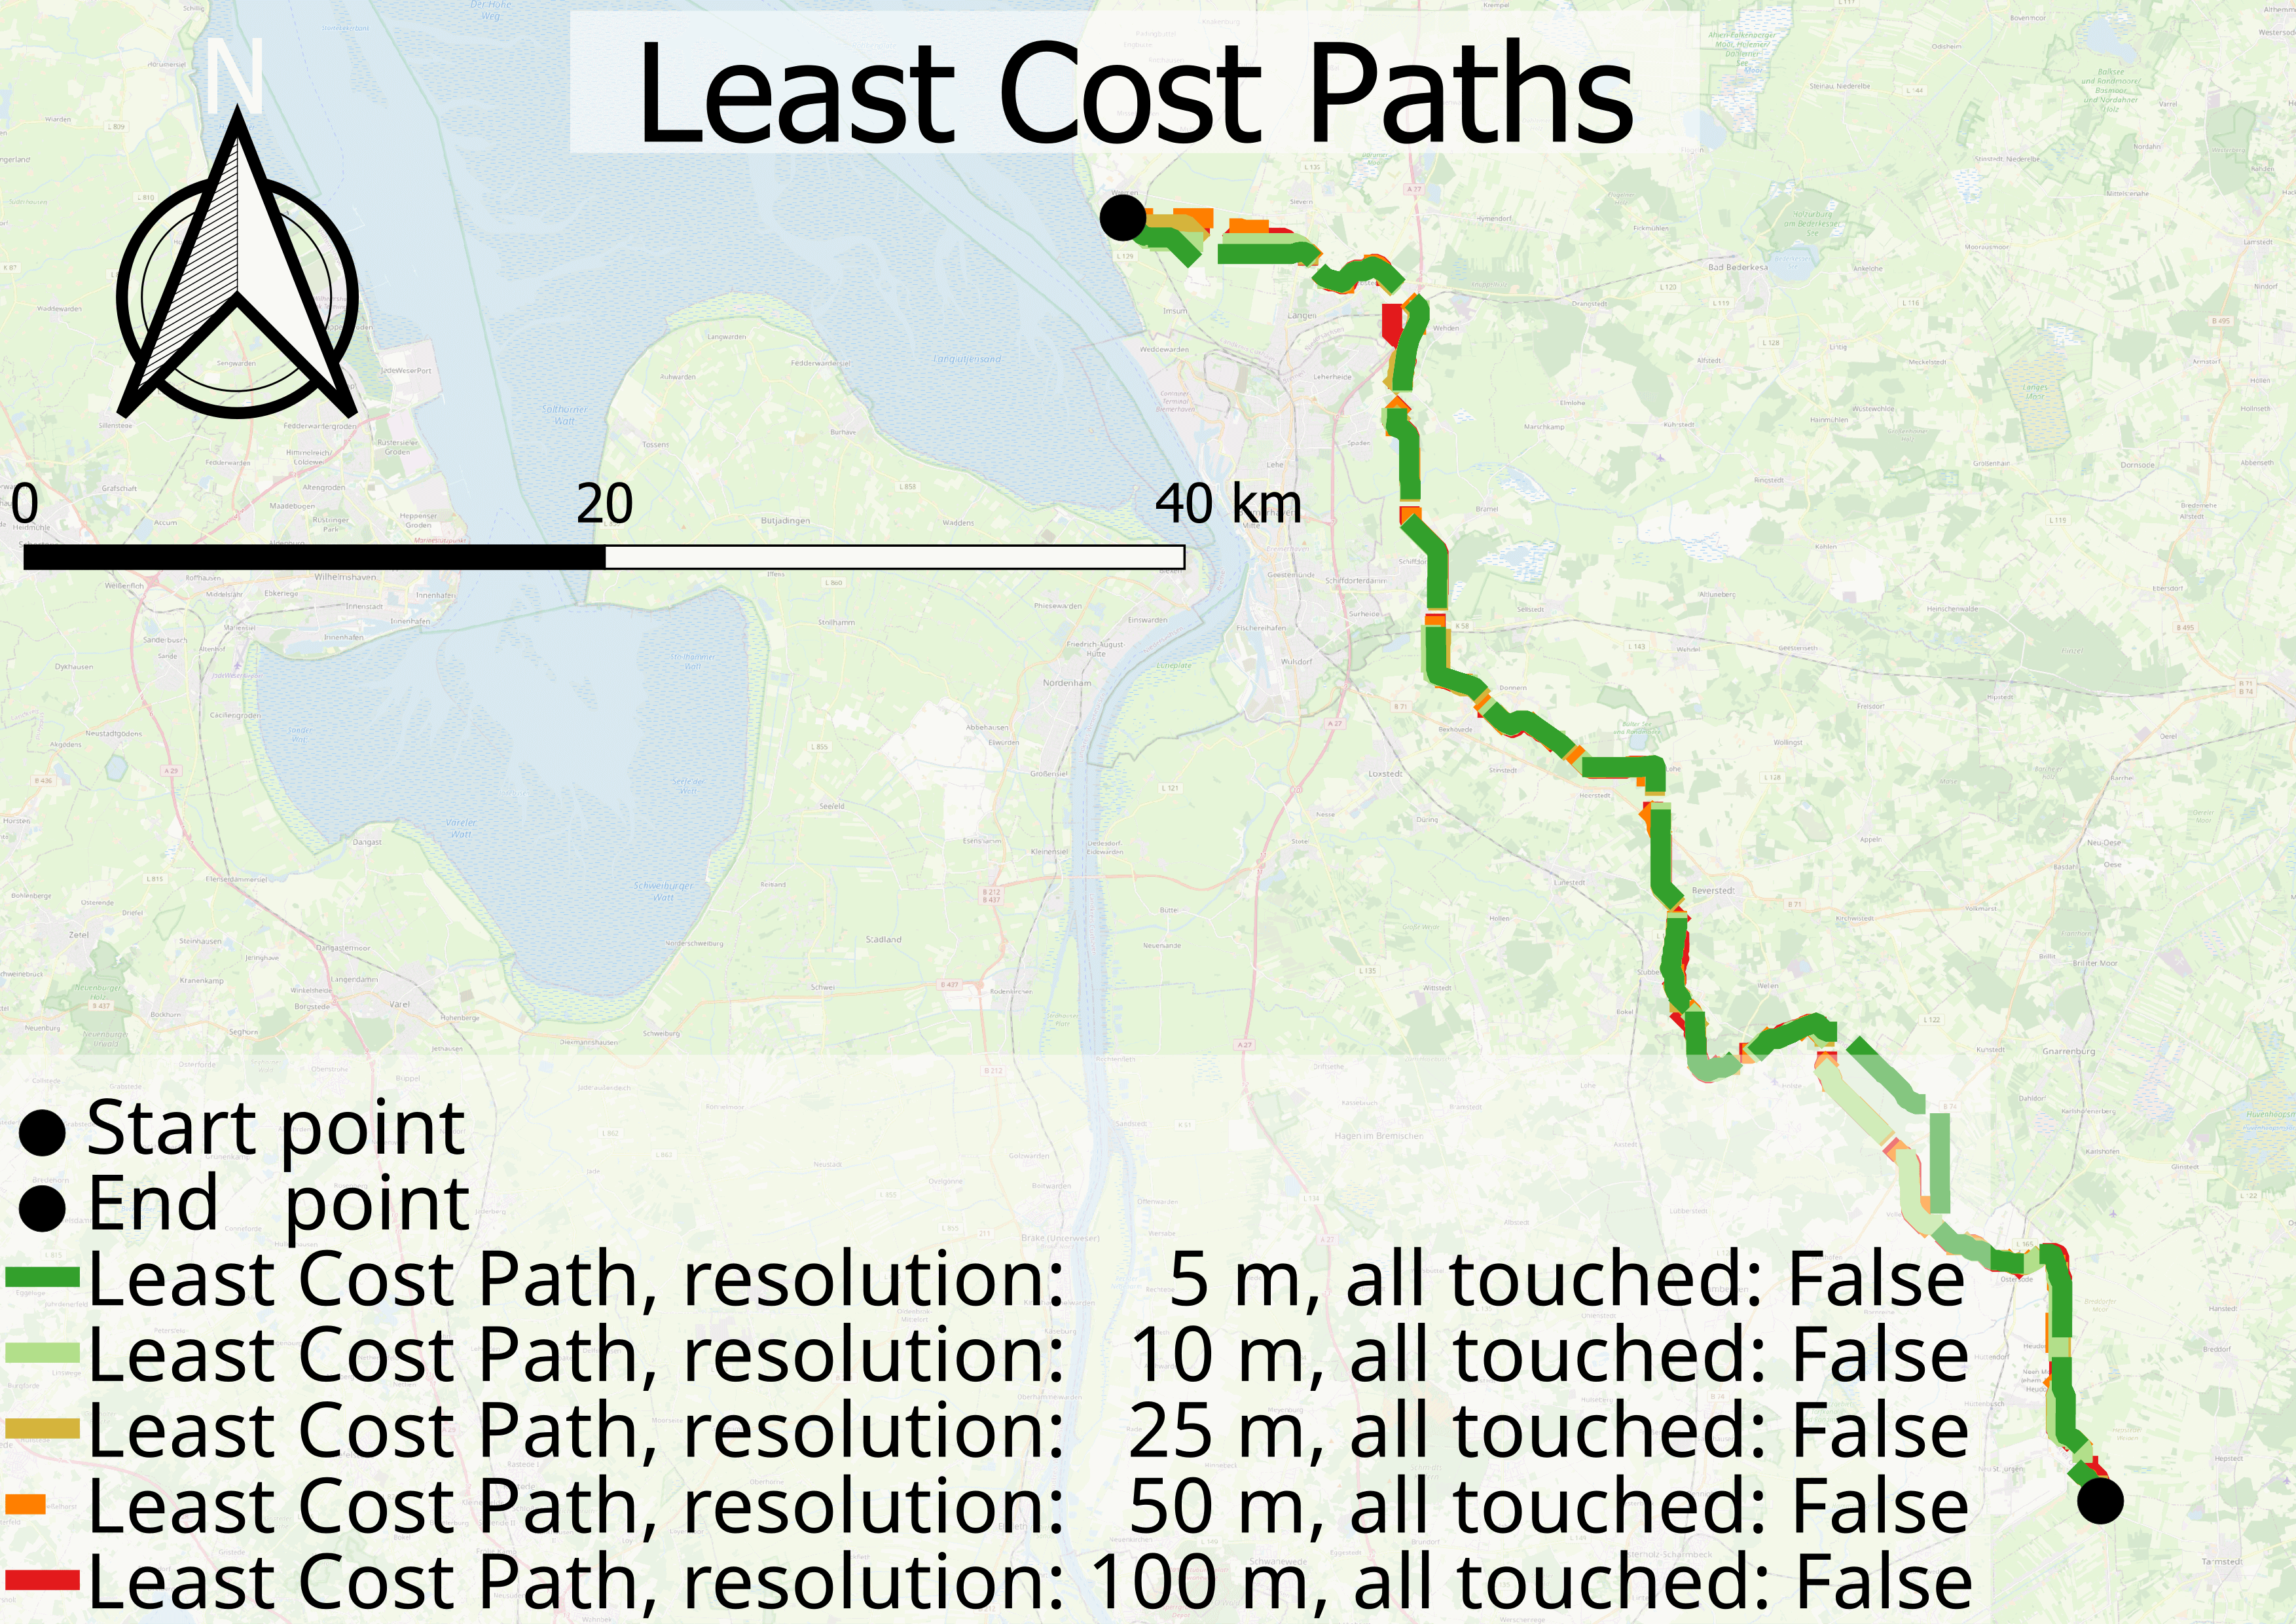
\includegraphics[width=.45\linewidth]{images/maps/LeastCostPaths_al_F_v2_small.png} }}%
			\qquad
			\subfloat[\centering all touched True.]{{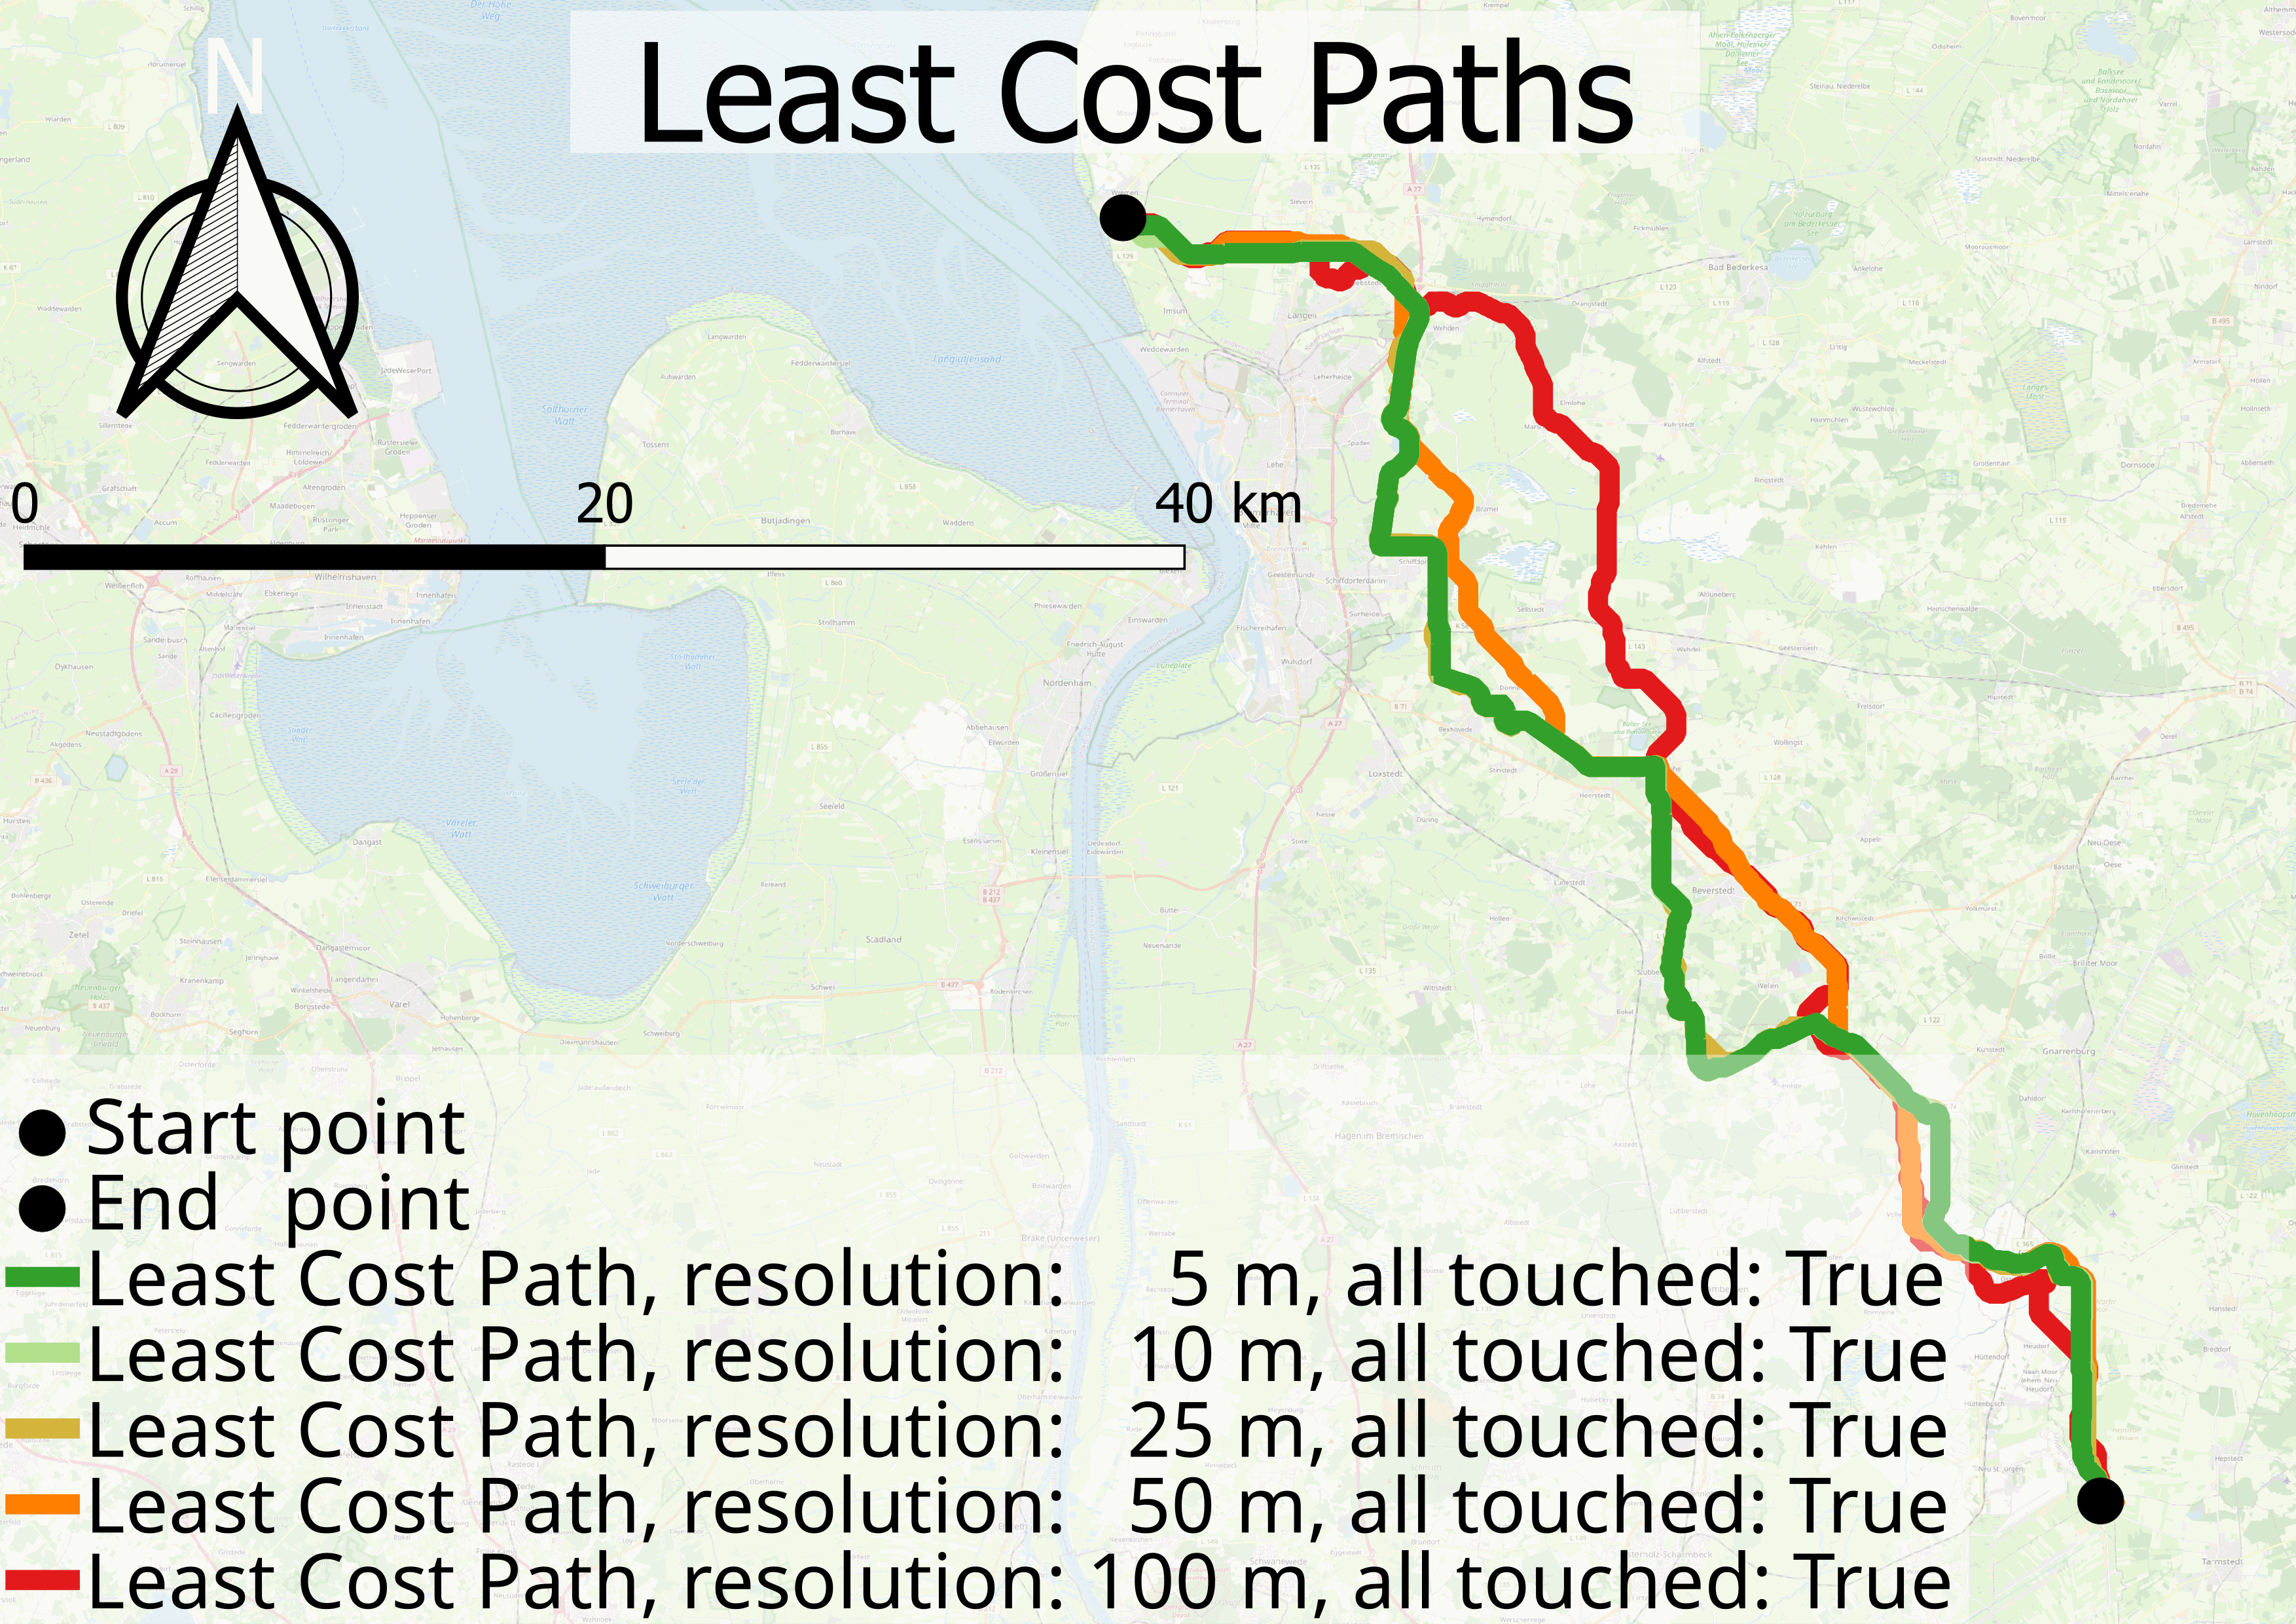
\includegraphics[width=.45\linewidth]{images/maps/LeastCostPaths_al_T_v2_small.png} }}%
			
			\caption{Figures of the Least Cost Paths, depending on the parameter all~touched. All~touched False: dashed lines, True: continuous lines. Gradation of resolutions: high (green) to low (red).}
			\label{fig:pathsAllTouched}
		\end{figure}
	\end{frame}

	\begin{frame}{Comparing: Costs}
		\begin{table}[t]
			\caption{Least Cost Paths: length~(l) for the different resolutions~(res), including the mean minimum distance~($d_{mean}$) and the agg. costs per resolution.} 
			\label{tab:2}
			\centering
			\begin{tabular}{ r  r  r  r  r  r   }
				res /m & $l_{al=f} /m$ & $l_{al=t} /m$ & $d_{mean}$ /m  & agg. $costs_{al=f} \times m$ & agg. $costs_{al=t} \times m$ \\
				\hline
				5 	& 76136.3	& 78002.0 &  126.0  & 93329.6 &  97584.8 \\
				10 	& 75430.1 	& 77936.6 &  277.9  & 89312.5 &  97311.8 \\
				25 	& 75422.9 	& 78422.9 &  313.8  & 83871.7 &  96816.4 \\
				50 	& 76135.0	& 70620.0 & 1140.0  & 70451.2 & 115003.7 \\
				100 & 76283.8	& 74120.7 & 1946.4  & 64051.6 & 167226.8 \\
			\end{tabular}
		\end{table}
	\end{frame}

\section{Speed-Up}
	\begin{frame}{Speed-Up: Clipping}
		\begin{figure}
			\centering
			
			\subfloat[\centering 50~m.]{{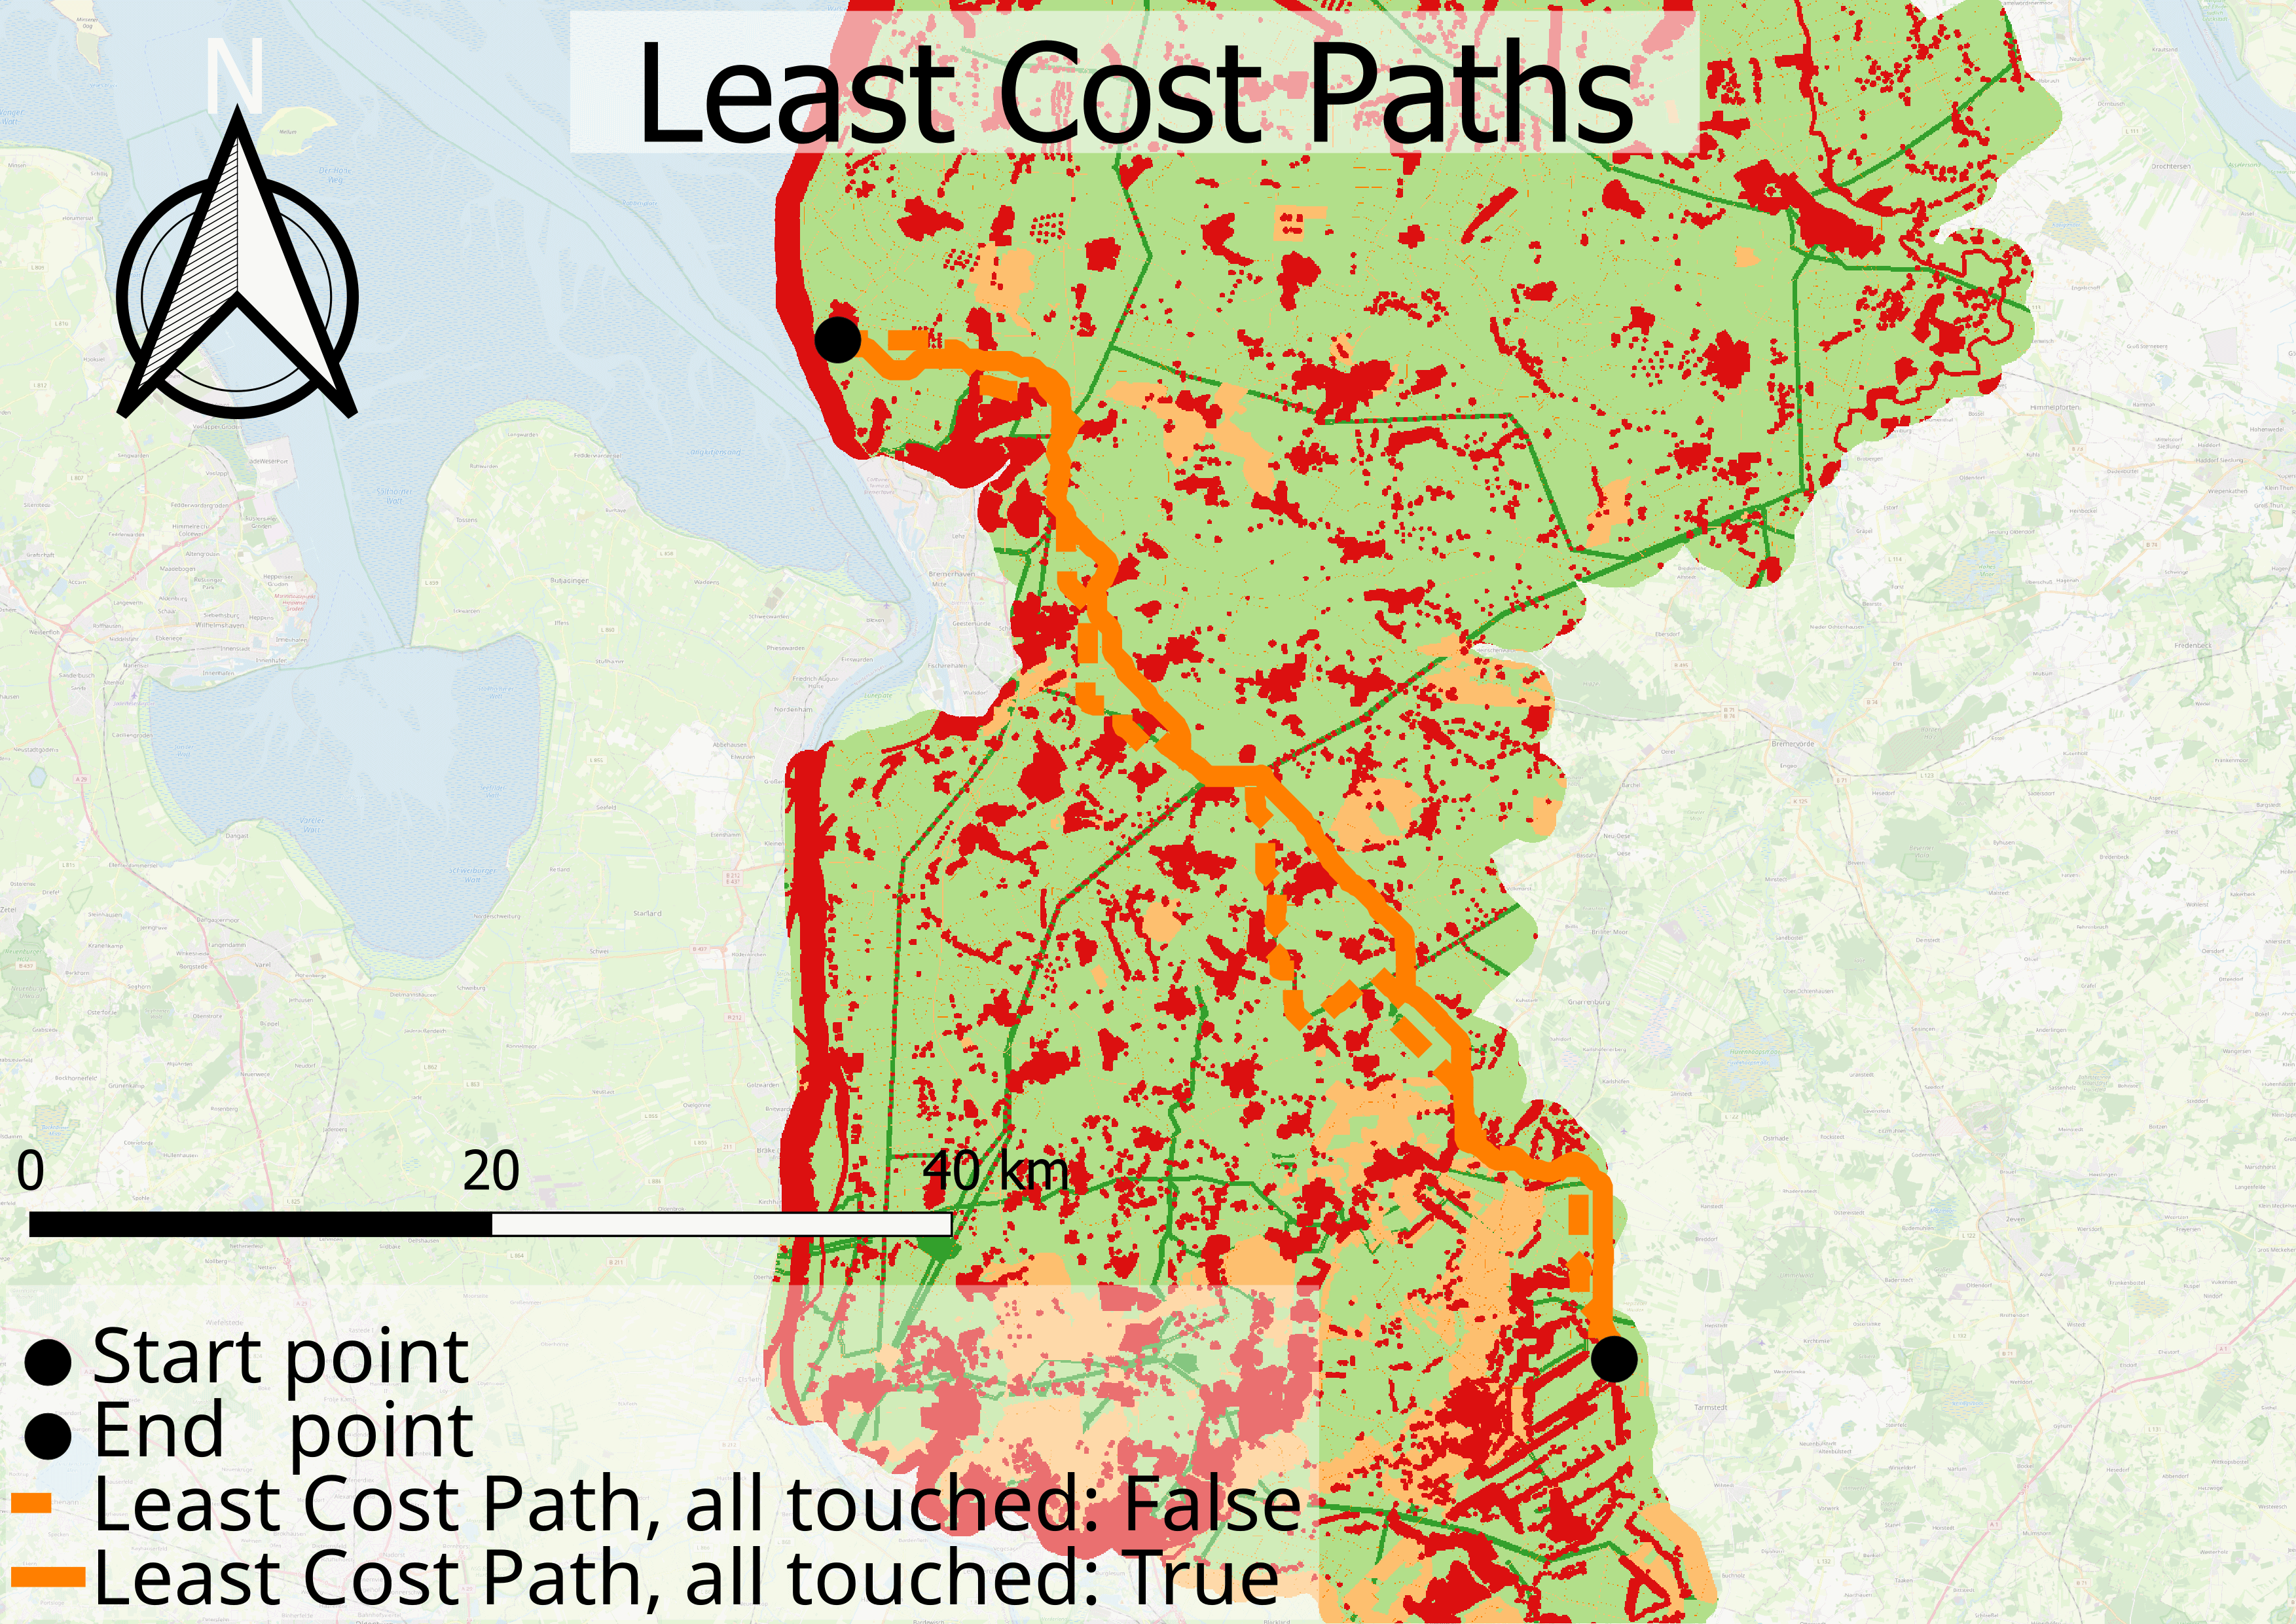
\includegraphics[width=.45\linewidth]{images/maps/LeastCostPath_50m_small.png} }}%
			\qquad
			\subfloat[\centering 5~m, clipped.]{{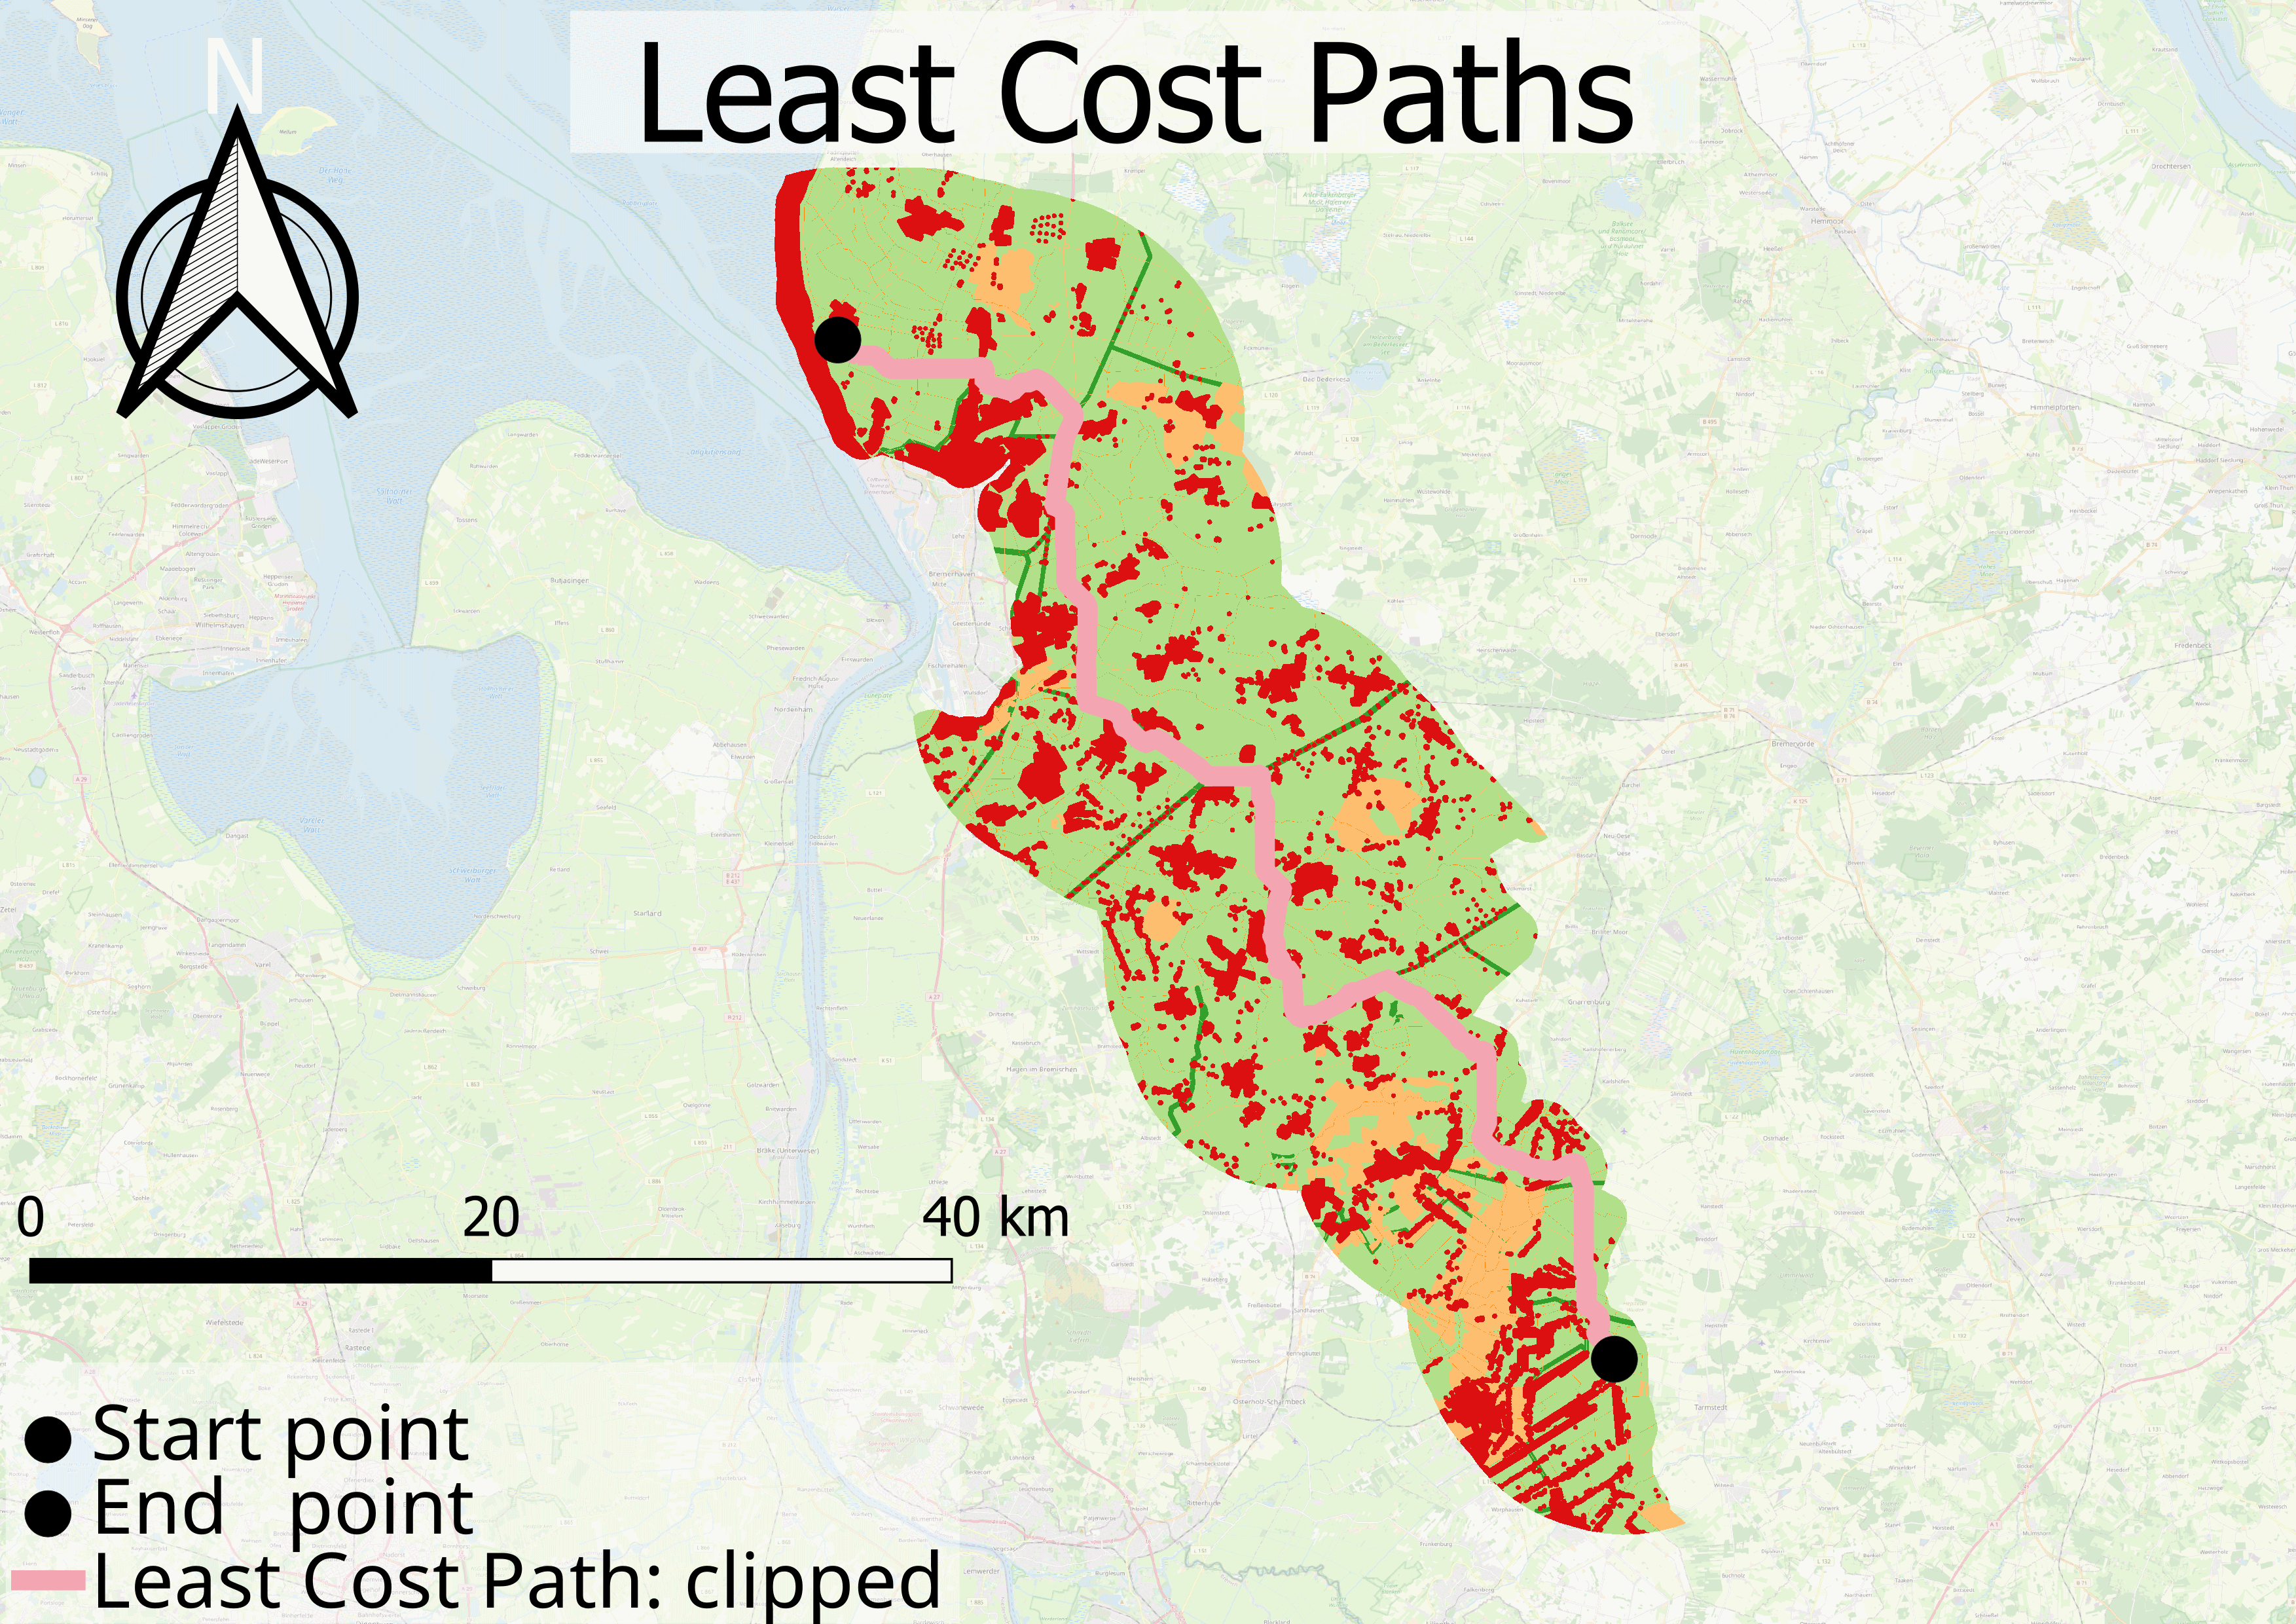
\includegraphics[width=.45\linewidth]{images/maps/LeastCostPath_5m_false_clipped_small.png} }}%
			
			\caption{Figures of the Least Cost Paths on the cost raster with 50~m resolution, used to clip the high resolution raster.}
			\label{fig:clipping}
		\end{figure}
	\end{frame}


	\begin{frame}{Speed-Up: Medium Resolution}
		\begin{minipage}[t]{0.48\textwidth}
		bi-linear down sampling
		\begin{itemize}
			\item 59.3~m average distance
			\item closer to path from all touched True
			
			\item independent from cost ratios
		\end{itemize}
		\end{minipage}
		\hfill	
		\begin{minipage}[t]{0.48\textwidth}
			weighted average cost raster
			\begin{itemize}
				\item best ration 4:1 False:True
				\item 40.1~m average distance
				\item closer to path from all touched True
				\item optimum: depends on cost ratio
			\end{itemize}
		\end{minipage}
	\end{frame}


	\begin{frame}{Speed-Up: Validation}
		\begin{minipage}[t]{0.48\textwidth}
			clipping
			\begin{itemize}
				\item reproduce-able best paths:\\ 3 times out of 4
				\item speed-up: unpredictable
			\end{itemize}
		\end{minipage}
		\hfill	
		\begin{minipage}[t]{0.48\textwidth}
			bi-linear down sampling
			\begin{itemize}
				\item distance worse than from original medium resolution
				\item speed-up: square of resolution
			\end{itemize}
		\end{minipage}
	\end{frame}

	\begin{frame}{Conclusion and Outlook}

	\begin{minipage}[t]{0.48\textwidth}
		conclusion
		\begin{itemize}
			\item provide Least Cost Path with WPS
			\item studied algorithmic speed-up
			     \begin{itemize}
			     	\item clipping
			     	\item medium resolution
			     \end{itemize}
		\end{itemize}
	\end{minipage}
	\hfill	
	\begin{minipage}[t]{0.48\textwidth}
		outlook
		\begin{itemize}
			\item non algorithmic speed-up
			\item set of possible paths
			\item stability: perturbation
		\end{itemize}
	\end{minipage}
	\end{frame}
\end{document}
